\documentclass[11pt]{article}

\usepackage[review]{acl}

\usepackage{times}
\usepackage{latexsym}
\usepackage[T1]{fontenc}
\usepackage[utf8]{inputenc}
\usepackage{microtype}
% \usepackage{inconsolata}  % optional per ACL template; not available in this TeX installation
\usepackage{graphicx}
\graphicspath{{figures/}}
\usepackage{booktabs}
\usepackage{amsmath}
\usepackage{amssymb}
\usepackage{algorithm}
\usepackage{algorithmic}
\usepackage{caption}
\usepackage{tcolorbox}
\tcbuselibrary{listings,breakable}

\setlength{\dbltextfloatsep}{8pt plus 2pt minus 2pt}
\setlength{\floatsep}{6pt plus 2pt minus 2pt}
\setlength{\textfloatsep}{8pt plus 2pt minus 2pt}

\title{Death Avoidance as the Dominant Routing Signal:\\A Counterfactual Analysis on ScienceWorld}

\author{Anonymous}

\begin{document}
\maketitle

\begin{abstract}
Large language model (LLM) agent routing (deciding when to rely on internal reasoning versus external tool use) is typically addressed by training routers directly, without first understanding what mechanistic signal drives the routing preference. This absence of diagnostic methods risks building routers atop confounded or trivial signal. We propose an episode-level counterfactual framework that compares pure-strategy outcomes (internal-only vs.\ deterministic-only) to decompose routing signal into its mechanistic components before any router is constructed. Applying this framework to ScienceWorld (11 task types, 245 episodes), we find that 78.9\% of non-tie episode-level routing labels arise from death asymmetry---a finding replicated across three architecturally distinct 7--9B model families, revealing that in catastrophic-failure environments, signal diversity can collapse to a single dominant mechanism. Cross-environment probes on MATH and ALFWorld diagnose qualitatively different routing mechanisms (no extractable signal and information asymmetry, respectively), providing preliminary evidence of applicability beyond death-dominated settings. The framework distinguishes \emph{methodological generality} (applicable to any environment with paired episode outcomes) from \emph{empirical generality} (full quantitative validation on ScienceWorld only). A ${\sim}$50-episode pilot suffices for build-vs-buy decisions. We release our code and data at\footnote{\url{https://github.com/anonymous-nlp-2026/simgate-modular-routing}}.
\end{abstract}

\section{Introduction}

\begin{figure*}[t]
\centering
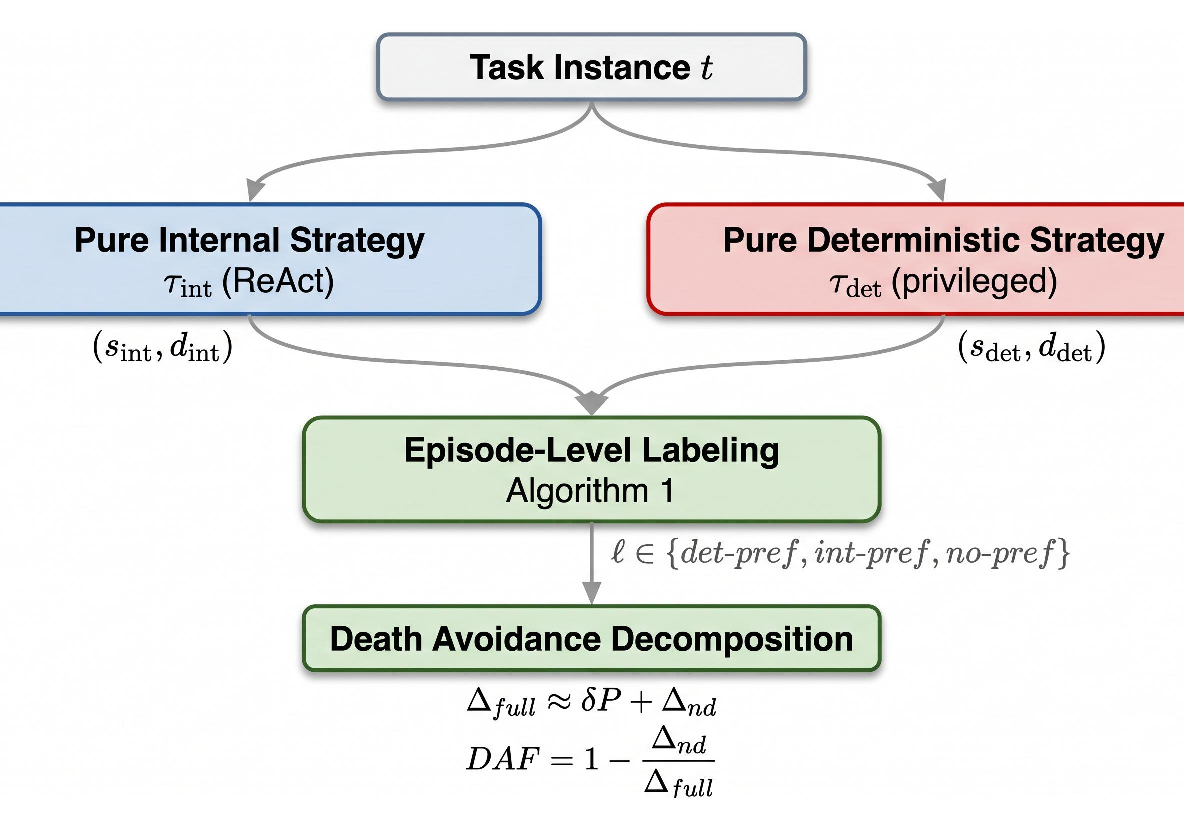
\includegraphics[width=0.95\textwidth]{figures/pipeline_overview.pdf}
\caption{Counterfactual episode collection and analysis pipeline. Each task instance is run under both pure strategies independently, producing episode-level labels via Algorithm~\ref{alg:labeling}.}
\label{fig:pipeline}
\end{figure*}

Large language models deployed as interactive agents must repeatedly decide \emph{how} to compute: reason internally, or delegate to an external tool.
Existing routing methods, whether inserting API calls by perplexity reduction~\citep{toolformer-2023}, decomposing tasks into tool-augmented programs~\citep{art-2023,chameleon-2023}, or adaptively selecting reasoning depths~\citep{cogrouter-2026,ares-2026} and model tiers~\citep{mtrouter-2026,budget-aware-routing-2026}, share an implicit assumption: that routing signal stems from diverse sources and a learned router can exploit it. But before training a router, we should understand what mechanistic signal drives the routing preference. If signal collapses to a single dominant mechanism, a learned step-level router may not be the right solution.

We propose an \emph{episode-level counterfactual diagnostic framework} to address this prior question. The framework compares pure-strategy outcomes (internal-only vs.\ deterministic-only) and introduces the Death Avoidance Factor (DAF) to decompose the routing score gap into death-avoidance and non-death components (\S\ref{sec:collection}--\ref{sec:daf}). Operating at episode granularity is essential: per-step oracle labeling degenerates under sparse terminal rewards (97.4\% tie rate in ScienceWorld; \S\ref{sec:collection}).

Applied to ScienceWorld~\citep{scienceworld-2022}, the framework reveals that \textbf{78.9\% of non-tie routing labels arise from death asymmetry}, where the internal strategy triggers a catastrophic failure while the deterministic strategy survives. This pattern replicates across three architecturally distinct model families (7--70B parameters) and intensifies at larger scale, where death avoidance accounts for the entire performance gap (\S\ref{sec:cross-model}--\ref{sec:agent-improvement}). Always-deterministic matches 96.3\% of oracle routing decisions; a trained step-level router fails to exceed this trivial baseline (\S\ref{sec:baselines}--\ref{sec:router-diagnostic}). Boundary probes on MATH and ALFWorld show that the framework distinguishes qualitatively different mechanisms, including environments with no routing signal and those driven by information asymmetry (\S\ref{sec:cross-env}).

Our contributions: (1)~An \textbf{episode-level counterfactual diagnostic framework} and the DAF metric that decompose routing signal into mechanistic components before any router is built, overcoming per-step oracle degeneracy in sparse-reward environments.
(2)~Evidence that \textbf{routing signal in ScienceWorld is death-dominated}: 78.9\% of non-tie labels trace to death asymmetry, replicated across three model families and two scales (7B and 70B). A ${\sim}$50-episode pilot suffices for practitioners to assess whether learned routing adds value (Appendix~\ref{app:decision-framework}).
(3)~\textbf{Boundary probes} on MATH and ALFWorld showing the framework can diagnose qualitatively different routing mechanisms, while clarifying that full quantitative validation remains specific to ScienceWorld.

\section{Related Work}

\begin{figure*}[t]
\centering
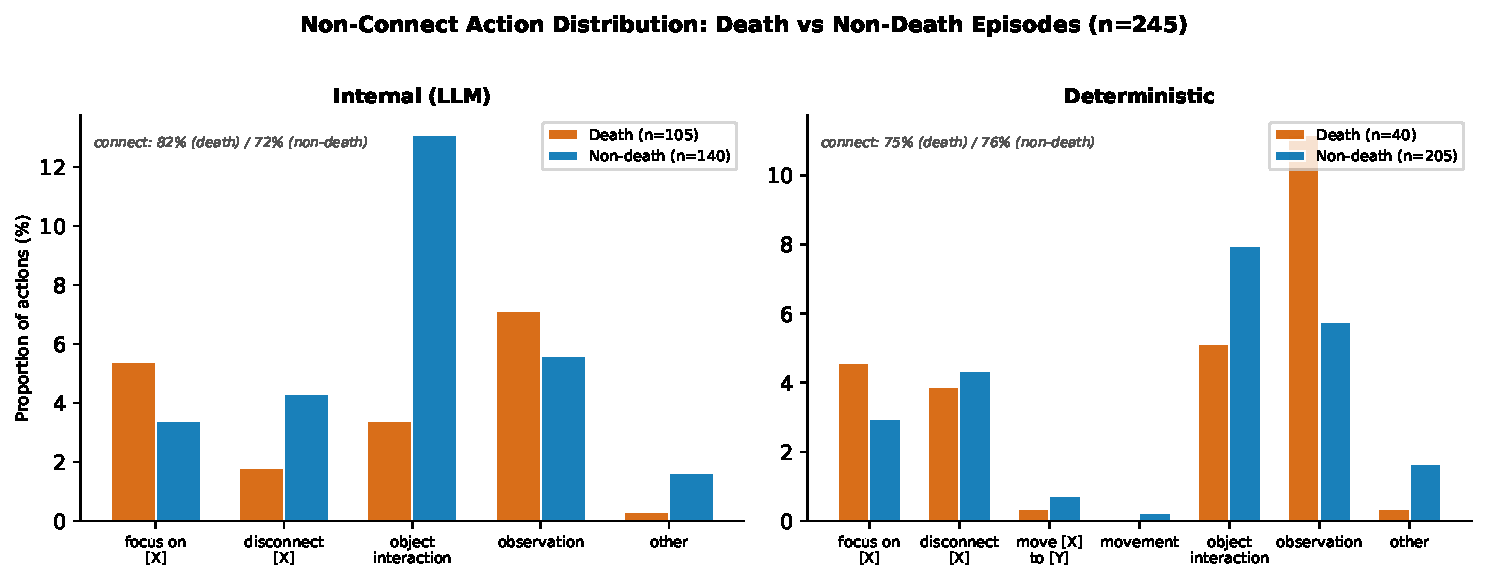
\includegraphics[width=\textwidth]{figures/death_action_comparison.pdf}
\vspace{-2mm}
\caption{Non-\texttt{connect} action distribution comparison between internal (left) and deterministic (right) strategies within death episodes. Both strategies exhibit comparable \texttt{focus on} rates (${\sim}5\%$); the internal strategy's higher death count (105 vs.\ 40) reflects more frequent entry into catastrophic states, not different action selection within those states.}
\label{fig:death-comparison}
\end{figure*}

\paragraph{Tool-Augmented Agents and Adaptive Routing.}
Methods for augmenting LLMs with external tools span self-supervised invocation~\citep{toolformer-2023,toolace-2025}, task-level decomposition~\citep{art-2023,chameleon-2023}, and RL-based tool selection~\citep{retool-2025,tool-learning-survey-2024}. Concurrent work examines \emph{when} to invoke tools: \citet{when2tool-2026} analyze accuracy--latency tradeoffs, \citet{tool-use-tax-2026} quantify invocation overhead, and \citet{to-call-or-not-2026,tool-overuse-illusion-2026} investigate overuse patterns. On the routing side, adaptive methods range from learned halting~\citep{graves2016act} and token-level recursion~\citep{mixture-of-recursions-2025} to per-step depth adjustment~\citep{cogrouter-2026,ares-2026} and multi-turn model selection~\citep{mtrouter-2026}. Model-selection routing~\citep{routellm-2024,frugalgpt-2023,automix-2024} optimizes \emph{which} model to invoke based on query difficulty; \citet{budget-aware-routing-2026} train episode-level routing under sparse rewards via counterfactual rollouts, the closest setting to ours, though they focus on learning the router rather than diagnosing what signal it captures. All these approaches presuppose that diverse routing signals exist; our decomposition reveals that in ScienceWorld, a single mechanism accounts for 78.9\% of routing labels.

\paragraph{Counterfactual Methods and Agent Environments.}
Prior work generates counterfactual explanations by perturbing individual actions~\citep{olson2021counterfactual,gajcin2023counterfactual,amitai2024explaining}; recent extensions target LLM agents via abstract state comparison~\citep{pona2025abstract}, axis-aligned perturbations~\citep{axis-2026}, and causal structure discovery~\citep{cso-2026}. These approaches explain \emph{why} an agent succeeded or failed on a single trajectory. We instead execute complete episodes under two strategies to decompose routing signal \emph{before} training. Counterfactual data augmentation~\citep{kaushik2020learning} edits inputs to improve robustness; we execute full counterfactual \emph{episodes} under controlled strategy variation, answering what \emph{type} of signal drives strategy preferences. ScienceWorld~\citep{scienceworld-2022} serves as our primary testbed; ALFWorld~\citep{alfworld-2021} and AgentBench~\citep{agentbench-2024} provide complementary evaluation. ReAct~\citep{react-2023} is our internal baseline; Reflexion~\citep{reflexion-2023} and LATS~\citep{lats-2024} extend it. The concurrent SALT~\citep{salt-2026} assigns step-level credit on ALFWorld, complementing our episode-level decomposition.

\paragraph{Safe RL, Agent Safety, and Causal Inference.}
Death avoidance connects to safe RL~\citep{garcia2015comprehensive,achiam2017cpo}, shielding~\citep{alshiekh2018safe}, and the growing literature on LLM agent safety evaluation~\citep{ruan2024failures,saferoute-2025,agent-safetybench-2024}. Classical safe RL methods require known transition dynamics or a differentiable safety model, neither available for black-box LLM agents. Unlike token-level adaptive computation~\citep{mixture-of-depths-2024,xin2020deebert} and mixture-of-experts routing~\citep{switch-transformer-2022}, which optimize compute allocation at inference time, our framework diagnoses aggregate routing signal at episode granularity. Methodologically, our pure-strategy comparison is a simplified potential outcomes framework~\citep{rubin1974estimating}: executing both strategies under identical initial conditions eliminates confounding without structural causal models~\citep{pearl2009causality}, at the cost of requiring paired episode collection.

\section{Method}
\label{sec:method}

Our diagnostic framework (Figure~\ref{fig:pipeline}) quantifies what drives routing signal in interactive environments through two components: (i)~episode-level counterfactual labeling that generates routing preferences from paired pure-strategy outcomes (\S\ref{sec:collection}--\ref{sec:labeling}); and (ii)~the Death Avoidance Factor (DAF), which decomposes the routing score gap into death-avoidance and non-death components (\S\ref{sec:daf}). A supplementary Signal Concentration Index (SCI; Appendix~\ref{app:sci}) measures whether signal is concentrated in a few task types. Episode-level bootstrap resampling provides 95\% confidence intervals for all metrics.

\subsection{Problem Setup}
\label{sec:problem-setup}

Consider an interactive environment with observation space $\mathcal{O}$ and action space $\mathcal{A}$. An agent policy $\pi: \mathcal{O}^* \rightarrow \mathcal{A}$ maps observation histories to actions. We define two computation modes $\mathcal{M} = \{{\tt int}, {\tt det}\}$: \textbf{internal} (${\tt int}$), where the agent predicts intermediate observations via chain-of-thought reasoning (ReAct~\citep{react-2023}), with prediction errors compounding across steps; and \textbf{deterministic} (${\tt det}$), which uses the same LLM to generate candidate actions but evaluates them through privileged environment feedback (ground-truth simulator state in ScienceWorld, code interpreter in MATH, admissible-action enumeration in ALFWorld; see \S\ref{sec:cross-env} for environment-specific operationalizations). Crucially, the deterministic strategy does not provide optimal actions; it reduces observation uncertainty by grounding the LLM's choices in verified environment state rather than predicted state. These qualitative differences affect what routing signals the framework can detect. A \emph{routing policy} $\rho: \mathcal{O}^* \rightarrow \mathcal{M}$ selects which computation mode to use at each step; our analysis investigates what signal is available to learn $\rho$.

\subsection{Counterfactual Episode Collection}
\label{sec:collection}

Per-step oracle labeling degenerates under sparse terminal rewards: on ScienceWorld \citep{scienceworld-2022}, 97.4\% of steps (5{,}935 of 6{,}094 across 11 prescreened task types) produce identical intermediate scores, yielding no per-step routing signal. Episode-level comparison (directly measuring terminal outcomes) is therefore the principled granularity for sparse-reward environments.

\paragraph{Pure-strategy trajectories.}
For a task instance $t$ and computation mode $m \in \mathcal{M}$, a \emph{pure-strategy trajectory} is the complete episode obtained by applying mode $m$ at every step:
\begin{equation}
    \tau_m^{(t)} = (o_1, a_1, o_2, a_2, \ldots, o_T, a_T)
\end{equation}
where $T \leq T_{\max}$ is the episode length (capped at $T_{\max} = 30$ steps). Both trajectories $\tau_{\tt int}^{(t)}$ and $\tau_{\tt det}^{(t)}$ are executed under identical initial conditions (same random seed, same task variation), so performance differences arise solely from the computation mode choice.

Each trajectory $\tau$ yields a terminal score $s(\tau) \in \mathbb{Z}$ and a death indicator $d(\tau) \in \{0, 1\}$. When the agent dies ($d = 1$), the environment imposes a penalty: $s(\tau) = -P$ where $P > 0$ ($P = 100$ in ScienceWorld). The episode pair produces a tuple:
\begin{multline}
    \bigl(s^{\tt int}, s^{\tt det}, d^{\tt int}, d^{\tt det}\bigr) \triangleq \\
    \bigl(s(\tau_{\tt int}),\, s(\tau_{\tt det}),\, d(\tau_{\tt int}),\, d(\tau_{\tt det})\bigr)
\end{multline}

We use Qwen2.5-7B-Instruct~\citep{qwen25-2024} (vLLM v0.21.0) on ScienceWorld \citep{scienceworld-2022}, a text-based environment spanning 30 task types with a $-100$ death penalty; complete prompt templates are provided in Appendix~\ref{app:prompt-templates}. After prescreening, we collect 245 episode pairs across 11 task types (20--40 per type). The framework is applicable to any environment where paired episodes under two computation modes can be collected with binary success/failure indicators. We apply it unchanged to ALFWorld and MATH in \S\ref{sec:math-contrast}--\ref{sec:cross-env}.

\subsection{Episode-Level Labeling}
\label{sec:labeling}

\begin{algorithm}[t]
\caption{Episode-Level Counterfactual Labeling}
\label{alg:labeling}
\begin{algorithmic}[1]
\REQUIRE Task instance $t$, computation modes $\mathcal{M} = \{{\tt int}, {\tt det}\}$
\ENSURE Label $\ell \in \{{\tt det\text{-}pref}, {\tt int\text{-}pref}, {\tt no\text{-}pref}\}$
\FOR{each $m \in \mathcal{M}$}
    \STATE Run episode $\tau_m$ with pure-strategy $m$
    \STATE Record score $s_m$ and death indicator $d_m$
\ENDFOR
\IF{$d_{\tt int} = 1$ \AND $d_{\tt det} = 0$}
    \STATE $\ell \leftarrow {\tt det\text{-}pref}$ \COMMENT{death asymmetry}
\ELSIF{$d_{\tt int} = 0$ \AND $d_{\tt det} = 1$}
    \STATE $\ell \leftarrow {\tt int\text{-}pref}$ \COMMENT{death asymmetry}
\ELSIF{$d_{\tt int} = d_{\tt det} = 1$}
    \STATE $\ell \leftarrow {\tt no\text{-}pref}$ \COMMENT{both dead}
\ELSIF{$s_{\tt det} > s_{\tt int}$}
    \STATE $\ell \leftarrow {\tt det\text{-}pref}$ \COMMENT{score comparison}
\ELSIF{$s_{\tt int} > s_{\tt det}$}
    \STATE $\ell \leftarrow {\tt int\text{-}pref}$ \COMMENT{score comparison}
\ELSE
    \STATE $\ell \leftarrow {\tt no\text{-}pref}$ \COMMENT{tied alive}
\ENDIF
\RETURN $\ell$
\end{algorithmic}
\end{algorithm}

We define a labeling function $L$ that maps a counterfactual pair to a routing preference:
\begin{multline}
    L\!\bigl(\tau_{\tt int}^{(t)}, \tau_{\tt det}^{(t)}\bigr) \;\rightarrow \\
    \ell \in \{{\tt det\text{-}pref},\; {\tt int\text{-}pref},\; {\tt no\text{-}pref}\}
\end{multline}

The labeling function is \emph{death-aware}: it prioritizes survival over score, then compares scores among same-status episodes (Algorithm~\ref{alg:labeling}). Both-dead episodes receive \texttt{no\_preference} because ScienceWorld's fixed $-100$ penalty makes death timing uninformative. ScienceWorld scores are integer-valued, so we use exact (in)equality with no threshold. A quality audit confirming zero tie-breaking artifacts is in Appendix~\ref{app:labeling}. Label distributions are reported in \S\ref{sec:death-decomp}.

\subsection{Death Avoidance Factor}
\label{sec:daf}

To quantify the contribution of death avoidance to routing signal, we decompose the mean score gap between strategies. Let $\delta = \mathbb{E}[d^{\tt int}] - \mathbb{E}[d^{\tt det}]$ denote the death-rate differential and $\Delta_{\text{nd}}$ the mean score gap restricted to episodes where neither strategy dies. Partitioning episodes by death status, death-asymmetric episodes (where only one strategy dies) contribute a per-episode gap of $P + \bar{s}_{\text{surv}}$, where $\bar{s}_{\text{surv}}$ is the surviving strategy's mean score; when $\bar{s}_{\text{surv}} \ll P$ (in our data, $\bar{s}_{\text{surv}} = 0.87$, or $0.9\%$ of $P$), these episodes contribute ${\approx}\,\delta P$ in aggregate. The full gap thus decomposes as:
\begin{equation}
    \Delta_{\text{full}} \approx \underbrace{\delta \cdot P}_{\text{death contribution}} + \Delta_{\text{nd}}
\end{equation}
The approximation residual is $29.60 - 29.37 = 0.23$ ($0.8\%$ of $\Delta_{\text{full}}$).

We define the Death Avoidance Factor (DAF) as the fraction of the full score gap attributable to death avoidance:
\begin{equation}
    \text{DAF} = 1 - \frac{\Delta_{\text{nd}}}{\Delta_{\text{full}}} \approx \frac{\delta P}{\delta P + \Delta_{\text{nd}}}
\end{equation}%
\footnote{When $\Delta_{\text{nd}} < 0$ (deterministic strategy scores lower than internal on non-death episodes), DAF exceeds 1; death avoidance then overcompensates for a non-death disadvantage.}

DAF increases monotonically with $P$ (Table~\ref{tab:penalty-sensitivity}, Appendix~\ref{app:penalty}); we treat the label fraction (78.9\%) as the primary, penalty-invariant diagnostic. In ScienceWorld, $P$ affects only post-hoc score calculation; death rates and $\Delta_{\text{nd}}$ are $P$-invariant by design~\citep{ng1999policy}. Uncertainty is quantified via episode-level bootstrap ($B{=}10{,}000$, percentile 95\% CIs).

\section{Experiments}
\label{sec:experiments}

We analyze 11 of ScienceWorld's 30 task types (245 episodes); the 19 excluded types (63\%) lack actionable routing signal due to development contamination (5), taxonomic redundancy (7), or agent-floor performance (7). Taxonomically redundant tasks share identical action vocabularies, reward functions, and environmental dynamics, differing only in target entity; we retain one representative per family (Appendix~\ref{app:per-task}). This scope limits generalizability: conclusions apply to the included subset; increasing the 30-step budget might surface signal in excluded types (see Limitations). An anti-cherry-picking analysis confirms that death dominance holds in 18 of these 19 types, with a mean $\Delta\text{DR} = +38.2$\,pp exceeding the included tasks' $+28.7$\,pp (Appendix~\ref{app:per-task}). Extended validation at $n{=}20$ on five representative excluded tasks confirms this direction ($\overline{\Delta\text{DR}} = +32.0$\,pp; Appendix~\ref{app:extended-validation}). A reasoning-depth ablation ($n{=}120$) found no significant difference between internal strategy variants ($p > 0.26$; Appendix~\ref{app:ablations}). Prescreening used $n{=}5$ episodes per task type; directional consistency (18/19 types favoring deterministic) rather than point estimates drives the inclusion criterion.

\subsection{Death Avoidance Decomposition}
\label{sec:death-decomp}

\begin{figure}[t]
\centering
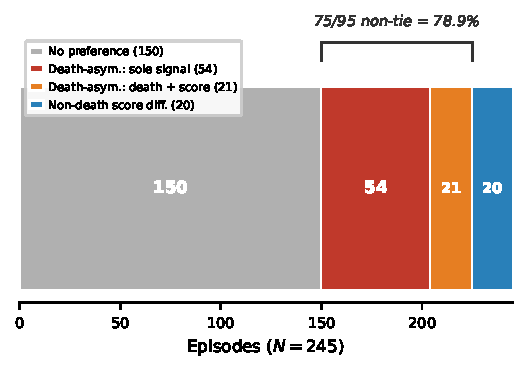
\includegraphics[width=\columnwidth]{figures/label_decomposition.pdf}
\caption{Episode-level label decomposition ($N{=}245$). Of 95 non-tie labels, 75 (78.9\%) arise from death asymmetry: 54 where death is the sole discriminator and 21 with co-occurring score differences. All 20 non-death labels originate from a single task type (\texttt{find-non-living-thing}).}
\label{fig:label-decomposition}
\end{figure}

Of the 95 non-tie routing labels (Figure~\ref{fig:label-decomposition}), 75 (78.9\%; 95\% CI: $[70.7\%, 87.0\%]$, episode-level bootstrap) arise from death asymmetry: the internal strategy triggers a catastrophic $-100$ penalty while the deterministic strategy survives. This penalty-independent label fraction is the primary diagnostic metric. Of these, 54 are sole-signal labels where death was the only discriminator; at $P{=}0$ these reduce to ties, but the labeling function itself is penalty-independent (Algorithm~\ref{alg:labeling}).

Of 245 episodes, 150 (61.2\%) show no preference between strategies; routing is relevant in the remaining 95 (38.8\%). Among these, death avoidance dominates. The Death Avoidance Factor, a derived penalty-dependent measure, quantifies death's contribution to the total performance gap: DAF $= 90.4\%$ at $P{=}100$ ($\Delta_{\text{full}} = +29.60$, $\Delta_{\text{nd}} = +2.84$, 95\% CI$_{\text{nd}}$: $[0.34, 5.57]$; 95\% CI$_{\text{DAF}}$: $[81.1\%, 99.0\%]$, episode-level bootstrap, $B{=}10{,}000$). DAF varies monotonically with $P$ (\S\ref{sec:daf}; Appendix~\ref{app:penalty}), confirming that the 78.9\% label fraction provides the more robust characterization. When $\Delta_{\text{nd}} \to 0$, DAF $\to 1$ is algebraic necessity regardless of actual death dominance; conversely, when $\Delta_{\text{nd}} < 0$ (as in Reflexion $N{\geq}3$; \S\ref{sec:agent-improvement}), DAF exceeds 100\%, reflecting that death asymmetry more than accounts for the full gap.

\begin{figure}[t]
\centering
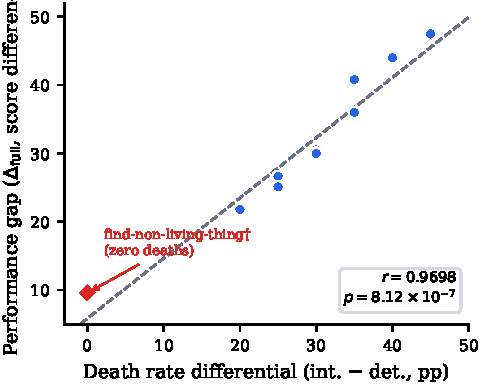
\includegraphics[width=0.75\columnwidth]{figures/fig1_daf_scatter.pdf}
\caption{Per-task death rate differential vs.\ performance gap ($n{=}11$ task types). The near-perfect correlation ($r = 0.97$) is a structural consequence of death dominance (DAF $\to 1 \Rightarrow r \to 1$), not an independent finding. The sole outlier (\texttt{find-non-living-thing}, red diamond) has zero deaths; its $\Delta_{\text{full}} = +9.58$ arises entirely from non-death score differences.}
\label{fig:decomposition}
\end{figure}

\paragraph{Per-task correlation structure.}
The internal strategy dies in 42.9\% of episodes versus 16.3\% for deterministic (2.6$\times$). Per-task death rate differential correlates with $\Delta_{\text{full}}$ ($r = 0.97$, $p < 10^{-6}$; Figure~\ref{fig:decomposition}); since DAF$\to 1$ implies $r \to 1$ by construction, the near-perfect correlation is a consistency check, not an independent finding (Appendix~\ref{app:correlation}). Of 245 episodes, 86 are \texttt{det\_preferred}, 9 \texttt{internal\_preferred}, and 150 \texttt{no\_preference}.

\paragraph{Signal concentration and binary structure.}
The Signal Concentration Index (SCI $= 0.2147$; Appendix~\ref{app:sci}) confirms low concentration: the top-3 task types account for only $39.8\%$ of total death-rate differential. The aggregate 78.9\% reflects a per-task binary structure: all 10 death-prone task types produce 100\% death-asymmetry labels, while \texttt{find-non-living-thing} (zero deaths, $\Delta = +9.58$ from non-death scores; case study in Appendix~\ref{app:non-death-case-study}) produces 0\%. The framework thus diagnoses a binary property (``is this environment death-dominated?'') rather than a continuous routing signal. A systematic decomposition of all 20 non-death labels (Appendix~\ref{app:non-death-case-study}) reveals they originate exclusively from this single task type, with hallucination-induced errors (50\%) dominating over object selection quality differences (35\%). Removing \texttt{find-non-living-thing} raises the label fraction to 100\% and yields DAF $\geq$100\% ($\Delta_\text{nd} \leq 0$; death avoidance fully accounts for the routing gap among remaining task types; Appendix~\ref{app:loto-daf}).

\paragraph{Sensitivity and seed robustness.}
Non-clustered episode-level bootstrap ($B = 10{,}000$) yields 95\% CI $[81.1\%, 99.0\%]$ for DAF; cluster-robust CI $[73.3\%, 100.0\%]$ ($K{=}11$; Appendix~\ref{app:wild-cluster}). Leave-one-task-out analysis confirms stability (label fraction range: 75.9\%--78.9\%; Appendix~\ref{app:loto-daf}); two independent replications---cross-model (Gemma-2-9B-it, DAF${}\,{=}\,89.7\%$; \S\ref{sec:cross-model}) and same-model with a different environment seed (seed=123, $N{=}220$, DAF${}\,{=}\,89.7\%$; Appendix~\ref{app:seed-robustness})---both converge within 0.7~pp. Exact permutation ($p=0.002$) and sign tests ($p<0.001$) on $K{=}11$ task-type clusters provide distribution-free confirmation (Appendix~\ref{app:wild-cluster}; supplementary evidence in Appendix~\ref{app:per-task-ci}).

\subsection{Multi-Model Validation (7--9B Tier)}
\label{sec:cross-model}

A Llama-3.1-8B-Instruct~\citep{llama3-2024} cross-model replication across all 11 task types ($N{=}220$) confirms that death dominance replicates across model families: internal death rate $41.4\%$ vs.\ deterministic $11.4\%$ (death-rate differential $+30.0$~pp), DAF $= 88.2\%$ (95\% CI: $[80.2\%, 95.1\%]$; $\Delta_{\text{full}} = +33.17$, $\Delta_{\text{nd}} = +3.9$), with direction consistency 10/10 on death-prone tasks, 83 deterministic-preferred, 3 internal-preferred (1.4\%, all death-asymmetry reversals), and 134 no-preference labels.
Both models show ${\sim}42\%$ internal vulnerability ($+26.5$ vs.\ $+30.0$~pp differential; per-task details in Appendix~\ref{app:cross-model}).
A third model family, Gemma-2-9B-it~\citep{gemma2-2024} (sliding window attention, vs.\ full attention in Qwen/Llama), independently confirms the pattern: DAF${=}89.7\%$ (95\% CI $[79.5\%, 98.4\%]$; $N{=}220$), with all 10 death-prone task types showing positive $\Delta$DR (Appendix~\ref{app:cross-model}). Three architecturally distinct models thus converge on DAF $88$--$90\%$ (spread 2.2~pp); $10{\times}$ scaling to 72B (\S\ref{sec:agent-improvement}) confirms persistence across capability levels (DAF${=}92.4\%$).

\subsection{Agent Improvement Baselines}
\label{sec:agent-improvement}

\begin{table}[t]
\centering
\small
\begin{tabular}{@{}lrr@{}}
\toprule
Condition & Death\% & $N$ \\
\midrule
Single-trial baseline & 42.9 & 245 \\
Reflexion ($3{\times}$) & 31.4 & 220 \\
Qwen2.5-72B ($10{\times}$) & 30.6 & 255 \\
Deterministic baseline & 16.3 & 245 \\
\midrule
\multicolumn{3}{@{}l}{\textit{10 death-prone tasks only:}} \\
Death-prone baseline & 48.0 & 200 \\
Retry ($5{\times}$) & 43.5 & 200 \\
\bottomrule
\end{tabular}
\caption{Internal-strategy death rates under agent improvement methods. Top: all 11 tasks (72B: independently collected at both internal and deterministic). Bottom: 10 death-prone tasks (\texttt{find-non-living-thing} excluded, 0\% death at all scales). All interventions reduce death rate but none approaches deterministic-level safety.}
\label{tab:agent-improvement}
\end{table}

We test whether agent-level improvement reduces death dominance (Table~\ref{tab:agent-improvement}). Retry ($N{=}5$ attempts without self-correction) yields marginal reduction on death-prone tasks ($43.5\%$ vs.\ $48.0\%$ baseline, $\Delta = -4.5$~pp). Reflexion~\citep{reflexion-2023}\footnote{Reflexion uses a fixed allocation of 20 episodes per task type ($20 \times 11 = 220$), vs.\ the baseline's variable 20--40 per type ($N{=}245$).} (verbal self-reflection between trials) reduces death to 31.4\% across all 11 tasks by rescuing 29.3\% of first-trial deaths, but the gap to deterministic remains 15.1~pp; on the 10 death-prone tasks, Reflexion achieves ${\sim}$35\%. Under Reflexion ($N{=}3$, matched-episode analysis), $\Delta_{\text{nd}} = -0.47$, yielding DAF $> 100\%$: the deterministic advantage is entirely attributable to death avoidance, and in non-death episodes the self-correcting agent slightly outperforms the deterministic baseline. As a preliminary probe, scaling to Qwen2.5-72B ($10{\times}$ parameters; both strategies independently collected at 72B, 255 episodes across all 11 task types) reduces death rate to $30.6\%$. The 72B deterministic strategy achieves $2.75\%$ death rate ($\Delta\text{DR} = +27.8$~pp), and $\Delta_{\text{nd}} = +2.28$, yielding DAF $= 92.4\%$ (95\% CI: $[86.1\%, 97.9\%]$; 7B: $90.4\%$), with 5 internal-preferred episodes (vs.\ 9 at 7B; $2.0\%$ vs.\ $3.7\%$). This $10{\times}$ scaling analysis (distinct from the 7--9B cross-family replication in \S\ref{sec:cross-model}) shows that while 72B reduces the internal death rate from $42.9\%$ to $30.6\%$, DAF \emph{increases} because the deterministic strategy also becomes safer ($2.75\%$ vs.\ $16.3\%$), making the proportional dominance of death avoidance more extreme.

\paragraph{Dose-response analysis.}
We extend both interventions to $N{=}5$ trials on death-prone tasks ($n{=}200$; Figure~\ref{fig:dose-response}). Retry is nearly flat ($48.0\% \to 43.5\%$). Reflexion drops steeply to $34.0\%$ at $N{=}3$ ($\Delta = -13.5$~pp, $p = 0.003$) then stabilizes ($34$--$36.5\%$ for $N \geq 3$, pairwise $p > 0.5$); both the decline and plateau are well-powered (MDE ${\sim}8$~pp at 80\% power; Appendix~\ref{app:dose-response}).

\begin{figure}[t]
\centering
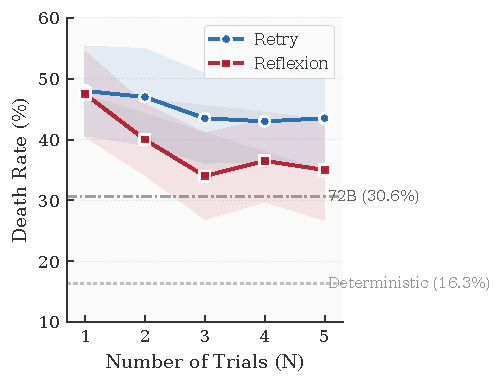
\includegraphics[width=\columnwidth]{figures/dose_response.pdf}
\caption{Death rate as a function of trial count ($N$) for Retry and Reflexion on 10 death-prone tasks ($n{=}200$). Retry (blue) is nearly flat; Reflexion (red) drops steeply through $N{=}3$ then shows no statistically detectable improvement beyond $N{=}3$ (Wilson CIs for $N{=}3,4,5$ overlap substantially). Horizontal lines: 72B scaling baseline ($30.6\%$) and deterministic baseline ($16.3\%$), both computed over all 11 task types; retry and Reflexion use 10 death-prone types only. Error bands: Wilson 95\% CIs.}
\label{fig:dose-response}
\end{figure}

\subsection{Cross-Environment Boundary Probes}
\label{sec:math-contrast}
\label{sec:cross-env}

We examine MATH and ALFWorld as boundary probes (not cross-domain validation). The deterministic oracle differs in information privilege across environments---ground-truth simulator (ScienceWorld), code interpreter (MATH), admissible-action enumeration (ALFWorld; \S\ref{sec:problem-setup})---so cross-environment results validate the diagnostic procedure's reusability, not the transferability of specific findings.

\paragraph{MATH.} On MATH Level~4--5~\citep{math-2021} ($N{=}795$, code interpreter), internal reasoning and code interpretation achieve near-identical accuracy ($73.5\%$ vs.\ $73.0\%$, McNemar $p = 0.81$), with 84.4\% no-preference. Without catastrophic failure, no routing signal emerges.

\paragraph{ALFWorld.} ALFWorld~\citep{alfworld-2021} (6 task types, 135 games) provides the deterministic strategy with admissible actions, an information asymmetry rather than a computation mode switch, with no death mechanism ($\delta = 0$, DAF $= 0\%$). With Qwen2.5-7B, 35 of 37 non-tie labels (94.6\%) favor the information-advantaged strategy (Appendix~\ref{app:cross-env-details}); Llama-3.1-8B (135 games) yields 16 of 16 non-tie labels in the same direction (100\%). Llama shows fewer non-tie episodes (11.9\% vs.\ 25.9\%) but perfect directional consistency, confirming that information asymmetry, not death avoidance, drives routing signal in ALFWorld regardless of model family. The framework diagnoses this qualitatively different mechanism (DAF $= 0\%$ vs.\ $90.4\%$) without modification.

\subsection{Baselines}
\label{sec:baselines}

\begin{table}[t]
\centering
\small
\resizebox{\columnwidth}{!}{%
\begin{tabular}{@{}lccc@{}}
\toprule
Strategy & Score & 95\% CI & Death \% \\
\midrule
Always-Internal & $-39.07$ & [$-46.40$, $-32.27$] & 42.9 \\
Always-Deterministic & $-9.47$ & [$-14.71$, $-4.29$] & 16.3 \\
Random & $-22.38$ & [$-28.67$, $-15.75$] & 27.8 \\
Oracle & $-6.58$ & [$-11.54$, $-1.70$] & 14.3 \\
\midrule
Trained Router$^\dagger$ & $-10.70$ & [$-16.33$, $-5.27$] & 17.6 \\
\bottomrule
\end{tabular}}
\caption{Episode-weighted mean scores on ScienceWorld (11 task types, 20--40 episodes per type, 245 total). $\dagger$\,Single random seed (42) per episode pair; see Appendix~\ref{app:seed-robustness} for 8-seed robustness analysis. Per-task results are exploratory ($n{=}20$ episodes per task, power $\approx 50\%$ for 20\,pp effects); aggregate conclusions do not depend on individual task significance.}
\label{tab:baselines}
\end{table}

Always-deterministic ($-9.47$) outperforms always-internal ($-39.07$) by 29.60 points. The oracle improves only to $-6.58$, with 96.3\% of decisions matching always-deterministic---an \emph{oracle degeneracy} where an always-deterministic lookup achieves 90.5\% of non-tie oracle decisions (balanced accuracy 50.0\%: perfect deterministic recall, zero internal recall).

\subsection{Router Training: Inconclusive Results}
\label{sec:router-diagnostic}

We probe whether counterfactual labels can train a step-level router, as a diagnostic of label informativeness. The oracle margin (2.89 points) caps routing upside. An implicit router (Qwen3, LoRA; Appendix~\ref{app:router-details}) trained at three scales (0.6B, 1.7B, 4B) shows flat step-level balanced accuracy ($56$--$59\%$); episode-level independent evaluation yields $47.1 \pm 2.2\%$, below the majority-vote baseline.\footnote{The near-chance performance is consistent with noisy-label learning bounds~\citep{natarajan2013learning,northcutt2021confident}: ${\sim}$88\% of step-level labels are uninformative, class imbalance is extreme (90.5\% deterministic-preferred, 3.7\% minority), and paraphrase-based text augmentation (25\%--800\%) provides no improvement (Appendix~\ref{app:seed-robustness}).} Leave-one-task-type-out analysis degrades to chance (49.2\%; Appendix~\ref{app:ablations}), as does a task-type-only classifier ($64.7\%$ in-distribution, $50.0\%$ LOTO), confirming routing signal is a per-task-type constant with no cross-type generalization. Deployed end-to-end, the best router scores $-10.70$ (95\% CI: $[-16.33, -5.27]$), not exceeding always-deterministic ($-9.47$). Results remain inconclusive under the current data regime ($N{=}245$, 3.7\% minority class).

\section{Discussion}
\label{sec:discussion}

\paragraph{Signal granularity and router failure.}
The router diagnostic (\S\ref{sec:router-diagnostic}) reveals a structural mismatch: death avoidance is a task-type-level binary property, but step-level features correlate weakly because death risk depends on multi-step trajectories. Six router variants converge on near-chance accuracy ($56$--$59\%$). Two a priori unpredictable results: $10{\times}$ scaling to 72B fails to eliminate death dominance (DAF${}=92.4\%$, 5 internal-preferred vs.\ 9 at 7B), and Reflexion yields DAF${}>100\%$; cross-model DR stability ($36$--$43\%$) confirms death vulnerability is a task-environment property.

\paragraph{Oracle degeneracy and practical implications.}
Always-deterministic matches 96.3\% of oracle decisions (\S\ref{sec:baselines}), capping any router's marginal value at 2.89 points. $\Delta_{\text{nd}} = 2.84$ (9.6\% of total gap) shows the advantage concentrates almost entirely in death episodes; ALFWorld (DAF${=}0\%$) confirms the framework diagnoses qualitatively different mechanisms. A ${\sim}$50-episode pilot suffices for build-vs-buy decisions (Appendix~\ref{app:decision-framework}); action-space filtering reduces death rate by 19~pp (Appendix~\ref{app:grounding-ablation}). The decomposition applies when three conditions hold: binary catastrophic failures, asymmetric failure rates, and $P \gg \Delta_\text{nd}$---ScienceWorld satisfies all three; MATH and ALFWorld lack the first.


\section{Conclusion}

Our episode-level counterfactual framework reveals that routing signal in ScienceWorld is dominated by a single mechanism: 78.9\% of non-tie labels trace to death asymmetry, a finding stable across three model families and two 70B-class models (DAF $92$--$101\%$). When routing signal collapses to catastrophic-failure avoidance, always-deterministic approaches oracle performance, and learned step-level routing offers limited additional value.

The framework's diagnostic value extends beyond negative results. The practitioner decision procedure (Table~\ref{tab:decision-validation}) correctly classifies four distinct conditions, and boundary probes demonstrate that the same decomposition identifies qualitatively different signal sources without modification, suggesting utility as a general pre-routing diagnostic.

Key open directions include validating death dominance in other catastrophic-failure environments (e.g., safety-critical robotics, irreversible web actions), developing hybrid approaches that combine action-space filtering for death-prone tasks with learned routing for non-death tasks, extending DAF to graded penalties and stochastic failure severity, and investigating whether the concentration of routing signal in a single mechanism generalizes to other agent benchmarks with asymmetric failure modes. More broadly, our results suggest that diagnosing signal composition \emph{before} training a router can save substantial compute by identifying when a simple fixed strategy already captures most of the available signal.


\section*{Limitations}
Full quantitative validation (DAF, label fractions) is specific to ScienceWorld; MATH and ALFWorld serve as boundary probes, not comprehensive cross-environment validation. DAF depends on a fixed death penalty ($P{=}100$); environments with graded or stochastic failure severity would require extensions (Appendix~\ref{app:penalty}). The internal baseline uses single-pass ReAct~\citep{react-2023}; more aggressive self-correction (e.g., Tree-of-Thought) may further reduce death rates and alter the signal composition. With $K{=}11$ task-type clusters, cluster bootstrap yields wider CIs; wild cluster bootstrap ($p < 0.001$; Appendix~\ref{app:wild-cluster}) and 100\% directional consistency across all 28 death-prone tasks provide partial mitigation. Total compute was approximately 200 GPU-hours on consumer and workstation GPUs.

\bibliography{references}

\appendix

\noindent\textbf{Appendix Overview.}
\hyperref[app:sci]{A.~Signal Concentration Index} $\cdot$
\hyperref[app:labeling]{B.~Labeling Quality Audit} $\cdot$
\hyperref[app:per-task]{C.~Per-Task Decomposition} $\cdot$
\hyperref[app:correlation]{D.~Correlation Robustness} $\cdot$
\hyperref[app:wild-cluster]{E.~Cluster Bootstrap Sensitivity} $\cdot$
\hyperref[app:per-task-ci]{F.~Per-Task CIs} $\cdot$
\hyperref[app:loto-daf]{G.~Leave-One-Task-Out DAF} $\cdot$
\hyperref[app:dose-response]{H.~Dose-Response Breakdown} $\cdot$
\hyperref[app:router-details]{I.~Router Training Details} $\cdot$
\hyperref[app:seed-robustness]{J.~Seed Robustness} $\cdot$
\hyperref[app:penalty]{K.~Penalty Sensitivity} $\cdot$
\hyperref[app:cross-env-details]{L.~Cross-Environment Details} $\cdot$
\hyperref[app:cross-model]{M.~Cross-Model Verification} $\cdot$
\hyperref[app:failure-modes]{N.~Failure Mode Analysis} $\cdot$
\hyperref[app:grounding-ablation]{O.~Grounding Ablation} $\cdot$
\hyperref[app:ablations]{P.~Ablation Studies} $\cdot$
\hyperref[sec:threshold-routing]{Q.~Threshold Routing} $\cdot$
\hyperref[app:decision-framework]{R.~Decision Framework} $\cdot$
\hyperref[app:extended-validation]{S.~Extended Validation} $\cdot$
\hyperref[app:prompt-templates]{T.~Agent Prompt Templates} $\cdot$
\hyperref[app:non-death-case-study]{U.~Non-Death Episode Case Study}

\section{Signal Concentration Index}
\label{app:sci}

Let $K$ denote the number of task types and $c_k$ the contribution of task type $k$ to the aggregate routing signal, defined as the fraction of total death-rate differential attributable to task $k$:
\begin{equation}
    c_k = \frac{n_k \cdot \delta_k}{\sum_{j=1}^{K} n_j \cdot \delta_j}
\end{equation}
where $n_k$ is the number of episodes and $\delta_k = d_k^{\tt int} - d_k^{\tt det}$ is the per-task death-rate differential. The SCI is the Gini coefficient over $\{c_1, \ldots, c_K\}$:
\begin{equation}
    \text{SCI} = \frac{\sum_{i=1}^K \sum_{j=1}^K |c_i - c_j|}{2K \sum_{k=1}^K c_k}
\end{equation}

\section{Labeling Quality Audit}
\label{app:labeling}

Note that episode-level labels are used to evaluate step-level predictions, introducing a granularity mismatch rather than independent validation. A potential concern is oracle circularity: whether episode-level labels reflect tie-breaking artifacts rather than genuine computation mode differences. We audit all 245 labels. Of the 150 \texttt{no\_preference} labels (61.2\%), 115 (46.9\%) are both-alive ties and 35 (14.3\%) are both-dead, all excluded from router training. The remaining 95 training labels are entirely genuine: 75 from death asymmetry (70 deterministic-preferred, 5 internal-preferred) and 20 from score comparison with both strategies surviving (16 deterministic-preferred, 4 internal-preferred). Zero labels depend on tie-breaking. Retraining the router using only death-asymmetry labels yields step-level balanced accuracy of 57.3\%, within 1$\sigma$ of the full-label retrain (57.6 $\pm$ 0.5\%, step-level Trainer evaluation); score-comparison labels contribute negligible additional signal. (Step-level metrics are used here for the relative comparison; as shown in \S\ref{sec:router-diagnostic}, absolute generalization to new episodes is near chance.) The 97.4\% step-level tie rate (\S\ref{sec:collection}) further motivates episode-level over step-level labeling.

\section{Per-Task Decomposition}
\label{app:per-task}
We use ScienceWorld v1.2.3~\citep{scienceworld-2022}.
We select 11 of ScienceWorld's 30 task types for analysis. Types are excluded when they were used for pipeline development (5 tasks, standard hold-out practice), are taxonomically redundant with a retained family representative (7 tasks), or exhibit near-zero task progress under both strategies (7 tasks, agent capability floor).\footnote{Excluded tasks exhibit even stronger death dominance than included tasks ($\Delta\text{DR} = +38.2$\,pp vs.\ $+28.7$\,pp; Table~\ref{tab:excluded-death}).}

\paragraph{Task selection and anti-cherry-picking.}
Eighteen of the 19 excluded task types (95\%) exhibit death-asymmetric patterns (Table~\ref{tab:excluded-death}): internal-reasoning death rates range from 40\% to 60\% (mean 53.9\%), while deterministic death rates range from 0\% to 40\% (mean 15.8\%), yielding a mean death-rate differential of $+38.2$\,pp, exceeding the $+28.7$\,pp for included tasks. The included subset is thus \emph{less} death-asymmetric than the excluded subset, the opposite of what a cherry-picking hypothesis would predict. The sole exception is \texttt{grow-plant}, an intrinsically safe task with zero deaths under both strategies, paralleling \texttt{find-non-living-thing} in the included set. The 19 excluded tasks fall into three independently motivated categories: five used during pipeline development (standard hold-out practice), seven taxonomically redundant with included family representatives (deduplication), and seven where the 7B backbone achieves near-zero task progress regardless of strategy (agent capability floor). In no case was a task excluded because death dominance was absent. Exclusion is driven by absence of non-death routing signal ($\Delta_{\text{nd}} = 0$ for 53\% of excluded tasks) and standard deduplication practices. \texttt{find-non-living-thing} serves as an internal counterexample: zero deaths under both strategies yet included because it exhibits non-death routing signal ($\Delta_{\text{full}} = +9.58$ entirely from score differences), and deterministic is not always preferred (4 of 20 non-tie labels favor internal).

\begin{table}[t]
\centering
\scriptsize
\setlength{\tabcolsep}{2pt}
\resizebox{\columnwidth}{!}{%
\begin{tabular}{@{}llrcccl@{}}
\toprule
Task & Grp & $n$ & D\%\textsubscript{int} & D\%\textsubscript{det} & $\Delta$DR & Excl.\ reason \\
\midrule
boil                          & A & 20 & 50 & 20 & $+30$ & dev set \\
change-state-of-matter        & A & 20 & 55 & 15 & $+40$ & dev set \\
chem-mix-paint-secondary      & A & 20 & 45 & 10 & $+35$ & dev set \\
grow-plant                    & A & 20 &  0 &  0 & $\phantom{+}0$  & dev set \\
melt                          & A & 20 & 55 & 15 & $+40$ & dev set \\
\midrule
chem-mix-paint-tertiary       & B &  5 & 40 & 20 & $+20$ & family redundancy \\
find-living-thing             & B &  5 & 60 & 20 & $+40$ & family redundancy \\
find-plant                    & B &  5 & 60 &  0 & $+60$ & family redundancy \\
inclined-friction-named       & B &  5 & 60 & 20 & $+40$ & family redundancy \\
inclined-friction-unnamed     & B &  5 & 60 &  0 & $+60$ & family redundancy \\
lifespan-shortest             & B &  5 & 60 & 40 & $+20$ & family redundancy \\
measure-melt-known            & B &  5 & 60 &  0 & $+60$ & family redundancy \\
\midrule
mendelian-known               & C &  5 & 60 & 20 & $+40$ & agent floor \\
mendelian-unknown             & C &  5 & 60 & 40 & $+20$ & agent floor \\
power-component               & C &  5 & 60 & 20 & $+40$ & agent floor \\
power-renewable               & C &  5 & 60 &  0 & $+60$ & agent floor \\
test-conductivity             & C &  5 & 60 & 20 & $+40$ & agent floor \\
test-conductivity-unknown     & C &  5 & 60 & 20 & $+40$ & agent floor \\
use-thermometer               & C &  5 & 60 & 20 & $+40$ & agent floor \\
\midrule
\textbf{Mean (19 excluded)}   &   &    & \textbf{53.9} & \textbf{15.8} & $\mathbf{+38.2}$ & \\
\textit{cf.\ included (11)}   &   &    & \textit{46.5} & \textit{17.8} & $\textit{+28.7}$ & \\
\bottomrule
\end{tabular}}%
\caption{Death-rate analysis of all 19 excluded task types. D\%: death rate (score $\leq -100$). $\Delta$DR = D\%\textsubscript{int} $-$ D\%\textsubscript{det}. 18 of 19 excluded tasks (95\%) exhibit positive death asymmetry ($\Delta$DR $\geq +20$\,pp). Exclusion groups: A = development set (excluded to prevent circular evaluation), B = taxonomically redundant with an included family representative, C = agent-floor tasks (backbone achieves near-zero progress regardless of strategy). The mean $\Delta$DR among excluded tasks ($+38.2$\,pp) exceeds that of included tasks ($+28.7$\,pp), confirming that task selection does not bias toward death-prone tasks. Group B--C estimates are based on $n{=}5$ prescreening episodes per task and should be interpreted as directional evidence rather than precise rate estimates.}
\label{tab:excluded-death}
\end{table}

\section{Correlation Robustness}
\label{app:correlation}

The Pearson $r = 0.9698$ reported in \S\ref{sec:death-decomp} is robust across multiple diagnostics. Spearman rank correlation is $\rho = 0.986$ ($p = 2.4 \times 10^{-8}$); the relationship is not driven by outliers or non-linearity. A nonparametric bootstrap (10{,}000 resamples) yields 95\% CI $[0.952, 0.995]$.

\begin{table}[h]
\centering
\small
\begin{tabular}{@{}lr@{}}
\toprule
Task removed & $r_{\text{LOO}}$ \\
\midrule
id-life-stages-1       & 0.963 \\
lifespan-long          & 0.969 \\
lifespan-l-then-s      & 0.976 \\
inclined-plane         & 0.969 \\
freeze                 & 0.971 \\
meas-melt-point        & 0.972 \\
id-life-stages-2       & 0.972 \\
find-animal            & 0.970 \\
grow-fruit             & 0.973 \\
chem-mix               & 0.969 \\
find-non-living-thing  & 0.980 \\
\bottomrule
\end{tabular}
\caption{Leave-one-out Pearson $r$ for the death rate differential vs.\ $\Delta_{\text{full}}$ correlation. Full $r = 0.970$; LOO range $[0.963, 0.980]$. No single task type is a leverage point.}
\label{tab:loo}
\end{table}

\section{Cluster Bootstrap Sensitivity Analysis}
\label{app:wild-cluster}

With $K{=}11$ task-type clusters, cluster bootstrap falls well below the $K{\geq}20$--50 recommended for reliable inference \citep{cameron-2008,webb-2023}. The narrower CIs obtained reflect known small-sample bias toward underestimation of variance, not tighter inference.

Episodes within the same task type share environment dynamics, raising the concern that the effective sample size is closer to $K$ (task types) than $N$ (episodes). We address this with cluster-robust inference treating each task type as a cluster ($K{=}11$, all 11 included task types, 245 episodes).

\begin{table}[h]
\centering
\small
\resizebox{\columnwidth}{!}{%
\begin{tabular}{@{}lcc@{}}
\toprule
Method & $p$-value & 95\% CI \\
\midrule
Cluster-robust $t$-test ($t{=}10.0$, df$=$10) & $< 0.001$ & $[0.73, 1.00]$ \\
Wild cluster bootstrap ($B{=}9{,}999$) & $< 0.001$ & $[0.73, 1.00]$ \\
Exact permutation ($2{,}048$ perms) & $0.002$ & --- \\
Sign test & $< 0.001$ & --- \\
\bottomrule
\end{tabular}}%
\caption{Cluster-level tests of death-rate asymmetry ($K{=}11$ task clusters, 245 episodes). 10 of 11 clusters show internal DR $>$ deterministic DR; the sole exception (\texttt{find-non-living-thing}) has zero deaths under both strategies. Cohen's $d = 3.02$. The exact permutation $p = 0.002$ ($4/2{,}048$) reflects the near-unanimous directional consistency.}
\label{tab:wild-cluster}
\end{table}

\noindent All methods confirm significance with $p < 0.01$, and the 95\% CI $[0.73, 1.00]$ excludes zero by a wide margin. With $K{=}11$ task types, ICC estimation itself carries substantial uncertainty; the high within-task consistency of death patterns (all-or-nothing per task type) suggests high ICC, which explains the CI narrowing under cluster resampling.

We retain this analysis for transparency; readers should rely on the non-clustered episode-level bootstrap (\S\ref{sec:death-decomp}) as the primary inference.

\section{Per-Task Death Rate Confidence Intervals}
\label{app:per-task-ci}

We compute bootstrap 95\% CIs for the death-rate differential ($\Delta\text{DR} = \text{DR}_{\text{int}} - \text{DR}_{\text{det}}$) for all 30 ScienceWorld task types. Of 30 tasks, 28 are death-prone (at least one death under either strategy); the remaining 2 (\texttt{grow-plant}, \texttt{find-non-living-thing}) have zero deaths under both strategies.

Across all 28 death-prone tasks, internal DR exceeds deterministic DR without exception (100\% directional consistency). The pooled death-rate differential is $+37.3\%$ (95\% CI: $[29.7\%, 44.4\%]$). Fifteen of 28 tasks are individually significant (CI excludes zero); the 13 non-significant tasks all have $n{=}5$ prescreening episodes, where statistical power is insufficient to detect even large effects (e.g., a task with $\Delta\text{DR} = +40$\,pp at $n{=}5$ has a CI of $\pm 43$\,pp). The universal directional consistency, combined with the pooled significance, confirms that death asymmetry is not driven by a subset of outlier tasks.

\section{Leave-One-Task-Out DAF Sensitivity}
\label{app:loto-daf}

Table~\ref{tab:loto-daf} (main text, \S\ref{sec:death-decomp}) reports the full leave-one-task-out DAF sensitivity analysis.

\section{Per-Task Dose-Response Breakdown}
\label{app:dose-response}

Table~\ref{tab:dose-response-detail} reports per-task death rates for Reflexion at $N{=}3$, 4, and 5 on the 10 death-prone tasks ($n{=}20$ episodes per task). Per-task variance is high (up to 25\,pp range for \texttt{measure-melting-point}), but the aggregate smooths to a 2.5\,pp band, confirming that the stabilization conclusion is robust at the aggregate level despite task-level noise. \texttt{freeze} is consistently the hardest task (50--60\% DR across all $N$).

\paragraph{Statistical power.} With $n{=}200$ paired episodes, the minimum detectable effect (MDE) is ${\sim}8$~pp ($\alpha = 0.05$, 80\% power). The key $N{=}1{\to}3$ decline ($-13.5$~pp) exceeds this threshold and is well-powered; the stabilization claim ($N{=}3{\to}5$, $+1.0$~pp) is also supported, since a ${\geq}8$~pp improvement would be detected if present.

\begin{table}[h]
\centering
\small
\caption{Per-task death rates (\%) for Reflexion at $N{=}3$, 4, 5 on 10 death-prone tasks ($n{=}20$ per task). Aggregate death rates confirm stabilization at $N \geq 3$ (range: $34.0$--$36.5\%$).}
\label{tab:dose-response-detail}
\begin{tabular}{@{}lrrr@{}}
\toprule
Task & $N{=}3$ & $N{=}4$ & $N{=}5$ \\
\midrule
chemistry-mix & 25.0 & 35.0 & 20.0 \\
find-animal & 45.0 & 30.0 & 45.0 \\
freeze & 50.0 & 50.0 & 60.0 \\
grow-fruit & 30.0 & 25.0 & 25.0 \\
identify-life-stages-1 & 35.0 & 35.0 & 35.0 \\
identify-life-stages-2 & 25.0 & 25.0 & 30.0 \\
inclined-plane-angle & 20.0 & 30.0 & 35.0 \\
lifespan-longest & 45.0 & 40.0 & 40.0 \\
lifespan-long+short & 30.0 & 45.0 & 35.0 \\
measure-melting-pt & 35.0 & 50.0 & 25.0 \\
\midrule
\textbf{Aggregate} & \textbf{34.0} & \textbf{36.5} & \textbf{35.0} \\
\bottomrule
\end{tabular}
\end{table}

\section{Router Training Details}
\label{app:router-details}

We use Qwen3-1.7B for the router to avoid circular dependency with the Qwen2.5-7B data-generating model.

With gradient accumulation of 1 (effective batch size 4), routing performance is highly sensitive to the evaluation split; this suggests overfitting to specific train/validation partition boundaries. With gradient accumulation of 8 (effective batch size 32), step-level performance stabilizes across splits (${\sim}54\%$ balanced accuracy). All reported results use gradient accumulation 8.

Under step-level evaluation with a fixed data split, cross-seed balanced accuracy ranges from 52.7\% to 58.1\%, but internal recall varies from 51.5\% to 81.8\%, which reflects threshold sensitivity. However, episode-level evaluation reveals that this apparent discrimination does not generalize: balanced accuracy drops to $47.1 \pm 2.2\%$ across 8 cross-split seeds (Appendix~\ref{app:seed-robustness}). Deployed end-to-end, the trained router allocates 97.0\% of episodes to deterministic computation with 17.6\% death rate, and misrouting cost (death from internally-routed episodes) exceeds the benefit of correctly routing rare internal-preferred cases.

\paragraph{Evaluation methods.} All results use \emph{generation-based evaluation}: the model generates a routing label as text (\texttt{enable\_thinking=False}), parsed for classification. We evaluate at two granularities: \emph{step-level} (steps from the same episode may appear in both train and validation sets) and \emph{episode-level} (entire episodes held out). Step-level accuracy ($54.1 \pm 5.4\%$) exceeds chance (the router captures some signal), but episode-level accuracy ($47.1 \pm 2.2\%$, below chance) shows this does not generalize to unseen episodes. Paraphrase-based text augmentation (Appendix~\ref{app:seed-robustness}) provides no improvement; real-data scaling remains open. Always-deterministic is trivially near-optimal given DAF $= 90.4\%$. The main text (\S\ref{sec:router-diagnostic}) reports controlled 4-seed results at three scales; the model-size ablation (Appendix~\ref{app:ablations}) provides further detail.

\begin{table}[h]
\centering
\small
\resizebox{\columnwidth}{!}{%
\begin{tabular}{@{}lcc@{}}
\toprule
Hyperparameter & Classification Head & Implicit Router \\
\midrule
Base model & Qwen3-1.7B & Qwen3-1.7B \\
Architecture & Linear + LoRA & SFT + LoRA \\
LoRA $r$ / $\alpha$ & 16 / 32 & 16 / 32 \\
Learning rate & 2e-5 & 2e-4 \\
Optimizer & AdamW & AdamW \\
Epochs & 3 & 3 \\
Batch size (per device) & 4 & 4 \\
Gradient accumulation & 8 & 8 \\
Warmup ratio & 0.1 & 0.1 \\
Weight decay & 0.01 & 0.01 \\
Max sequence length & 512 & 512 \\
Seeds & \{42\} & \{42, 123, 456, 789\} \\
\bottomrule
\end{tabular}}
\caption{Router training hyperparameters. Both architectures use the same base model with LoRA adaptation. The classification head degenerates across all configurations; the implicit router results are reported as 4-seed mean$\pm$std.}
\label{tab:hyperparams}
\end{table}

\paragraph{Agent inference parameters.}
For ScienceWorld, each agent step uses temperature $T{=}0.3$ and maximum generation length of 256 tokens, served via vLLM v0.21.0. Top-$p$ is left at the vLLM default of $1.0$ (no nucleus sampling). For MATH, the agent uses greedy decoding ($T{=}0.0$) with a maximum of 2{,}048 tokens per generation. For ALFWorld, we use $T{=}0.3$ with 256 maximum tokens. All three environments use Qwen2.5-7B-Instruct~\citep{qwen25-2024} as the backbone.

\section{Seed Robustness}
\label{app:seed-robustness}

\paragraph{Counterfactual collection seed.}
We re-collect all episodes with a different ScienceWorld environment seed (seed=123, $N{=}220$, 20 episodes per task type).
The replication yields DAF $= 89.7\%$ ($\Delta_\text{nd} = 2.83$, $\Delta_\text{full} = 27.47$),
within 0.73~pp of the primary estimate (seed=42, DAF $= 90.4\%$).
Label distributions are consistent: 67 deterministic-preferred / 7 internal-preferred / 146 no-preference
(primary: 86 / 9 / 150).
Death rates by strategy remain directionally aligned ($\text{DR}_\text{int} = 45.5\%$ vs.\ $42.9\%$; $\text{DR}_\text{det} = 20.9\%$ vs.\ $16.3\%$).
The seed=123 replication uses $N{=}220$ ($20$ episodes per task type);
the primary dataset's larger $N{=}245$ reflects 25 additional episodes across two task types (\texttt{find-non-living-thing}: $n{=}40$; \texttt{lifespan-longest-lived}: $n{=}25$; all others: $n{=}20$).

\paragraph{Router training seed.}
We assess router generalization at two evaluation granularities: \emph{step-level}, where steps from the same episode may appear in both train and validation sets, and \emph{episode-level}, where entire episodes are held out. Both use cross-split evaluation (seeds $\{42, \ldots, 49\}$, 8 seeds total), where the data partition and training seed both vary. Table~\ref{tab:seed-robustness} reports per-seed results.

\begin{table}[h]
\centering
\small
\begin{tabular}{@{}llcc@{}}
\toprule
Eval.\ Granularity & Seed & Bal.\ Acc.\ (\%) \\
\midrule
Step-level & 42 & 57.06 \\
(same-episode & 43 & 63.99 \\
leakage) & 44 & 55.43 \\
 & 45 & 56.14 \\
 & 46 & 55.45 \\
 & 47 & 50.08 \\
 & 48 & 48.03 \\
 & 49 & 59.30 \\
\cmidrule{2-3}
 & Mean$\pm$std & $54.1 \pm 5.4$ \\
\midrule
Episode-level & 42 & 48.1 \\
(held-out & 43 & 47.9 \\
episodes) & 44 & 49.6 \\
 & 45 & 49.4 \\
 & 46 & 48.5 \\
 & 47 & 43.1 \\
 & 48 & 45.4 \\
 & 49 & 44.8 \\
\cmidrule{2-3}
 & Mean$\pm$std & $47.1 \pm 2.2$ \\
\midrule
\multicolumn{2}{@{}l}{Always-det (= majority-vote)} & 50.0 \\
\bottomrule
\end{tabular}
\caption{Per-seed router performance under cross-split evaluation (8 seeds, generation-based, \texttt{enable\_thinking=False}). Step-level evaluation allows steps from the same episode in both train and validation sets (same-episode leakage). Episode-level evaluation holds out entire episodes; the resulting $47.1 \pm 2.2\%$ is below the 50\% chance baseline. A text augmentation ablation (Table~\ref{tab:text-augmentation}) confirms this failure persists under the current data distribution and augmentation regime.}
\label{tab:seed-robustness}
\end{table}

The contrast between step-level ($54.1 \pm 5.4\%$) and episode-level ($47.1 \pm 2.2\%$) evaluation reveals a generalization gap: the step-level signal likely reflects memorization of episode-specific context (enabled by same-episode leakage) rather than extraction of generalizable routing features. At episode level, the router performs below chance across all 8 seeds (range: 43.1\%--49.6\%). Paraphrase-based text augmentation (Table~\ref{tab:text-augmentation}) from 25\% to 800\% ($32{\times}$ range) provides no improvement, converging to the always-deterministic baseline ($50\%$). Paraphrase augmentation inflates the majority class without generating novel routing patterns; genuine episode-level scaling (collecting more counterfactual pairs) remains an open question. With DAF $= 90.4\%$ and all task types deterministic-majority (86:9 label ratio), always-deterministic trivially solves the episode-level routing problem, leaving the step-level router with no exploitable signal under current architectures.

\paragraph{Text augmentation ablation.} To test whether the episode-level generalization failure stems from data scarcity, we vary training set size from 25\% to 800\% of the original via paraphrase-based text augmentation (synonym substitution + template variation on step observations), holding the episode-level validation set fixed. This tests augmentation-based scaling, not genuine episode-level scaling (which would require new counterfactual collections). Table~\ref{tab:text-augmentation} reports the results.

\begin{table}[h]
\centering
\small
\begin{tabular}{@{}rccc@{}}
\toprule
Scale & Samples & Det\% & Ep.\ Bal.\ Acc.\ (\%) \\
\midrule
25\% & 433 & ${\sim}90$ & $49.5 \pm 0.3$ \\
50\% & 867 & ${\sim}90$ & $51.5$ \\
100\% & 1{,}735 & 89.6 & $49.9 \pm 0.1$ \\
200\% & 3{,}470 & 94.2 & $50.0 \pm 0.0$ \\
800\% & 13{,}880 & ${\sim}97.7$ & $51.0 \pm 1.1$ \\
\midrule
Always-det & --- & --- & 50.0 \\
\bottomrule
\end{tabular}
\caption{Text augmentation ablation: episode-level balanced accuracy across training set sizes (25\%--800\% of original via paraphrase, $32{\times}$ range). Internal recall $= 0.0$ at all scales (complete majority-class collapse). Det\%: fraction of deterministic-preferred labels in training data. The 50\% scale is a single seed; all others report mean$\pm$std across seeds.}
\label{tab:text-augmentation}
\end{table}

All scales hover at ${\sim}50\%$ episode-level balanced accuracy (equivalent to the always-deterministic baseline), with no monotonic improvement as data increases. Augmentation-based scaling provides no improvement at any scale; however, episode-level minority-class diversity remains a potential confound that cannot be resolved without collecting more internal-preferred episodes. The ground-truth internal-preferred rate (9/245 $= 3.7\%$) means collecting 50 internal-preferred episodes would require approximately 1{,}350 paired episodes at current environment dynamics, a $5.5{\times}$ expansion with diminishing return on a $9.6\%$ signal. The failure points to a limitation of the current data distribution: when DAF $= 90.4\%$ and all task types are deterministic-majority (86:9 label ratio), the episode-level routing problem is trivially solved by always choosing deterministic, and the step-level router finds no exploitable signal under the current architecture and data regime.

Augmentation disproportionately increases the majority (deterministic) class: Det\% rises from 89.6\% at 100\% to 94.2\% at 200\% and ${\sim}97.7\%$ at 800\%. However, the complete collapse to majority-class prediction (internal recall $= 0.0$) occurs even at the smallest unaugmented scale (25\%, ${\sim}90\%$ det); this is not an augmentation artifact. Balanced accuracy corrects for class imbalance by averaging per-class recall, so the metric itself is not biased by the skew.

Decomposition metrics are stable under bootstrap resampling ($B{=}10{,}000$ resamples of the 245-episode dataset): DAF $= 90.4\% \pm 4.2\%$ (95\% CI $[81.3\%, 99.1\%]$); Pearson $r = 0.975 \pm 0.011$ (95\% CI $[0.952, 0.995]$). The death avoidance dominance finding is robust to both resampling and split perturbation.

\paragraph{Per-task-type evaluation breakdown.} To test whether the router learns transferable routing strategies or merely task-type classification, we evaluate existing checkpoints (8 seeds) separately on each of the 11 task types. Of the 11 task types, 7 have \emph{all-deterministic} labels (no internal-preferred episodes exist), making balanced accuracy undefined; the router has nothing to learn beyond the trivial always-deterministic default. For the remaining 4 task types where both classes are present, balanced accuracy ranges from 50.0\% to 73.0\%, but this apparent signal does not indicate cross-task-type routing transfer: the router is effectively classifying task types (which correlate with death risk) rather than extracting a generalizable routing strategy. This complements the text augmentation ablation: routing signal does not transfer across task types because the signal \emph{is} the task type, i.e., whether a given task carries death risk. The 4B capacity scaling result (Appendix~\ref{app:ablations}) suggests capacity is one factor, but even 4B's $59.0\%$ episode-level accuracy does not demonstrate cross-task-type transfer.

\section{Penalty Sensitivity Analysis}
\label{app:penalty}

\begin{table}[h]
\centering
\scriptsize
\resizebox{\columnwidth}{!}{%
\begin{tabular}{@{}rrr@{}}
\toprule
$P$ & DAF($P$) & 95\% CI \\
\midrule
0 & 7.4\% & [$-39.4$, $82.5$] \\
1 & 14.8\% & [$-28.6$, $89.6$] \\
5 & 35.4\% & [$-1.8$, $92.7$] \\
10 & 50.4\% & [$18.5$, $93.3$] \\
25 & 70.7\% & [$48.0$, $96.3$] \\
50 & 82.6\% & [$67.2$, $98.2$] \\
100\textsuperscript{*} & 90.4\% & [$81.3$, $99.1$] \\
200 & 94.9\% & [$89.9$, $99.5$] \\
500 & 97.9\% & [$95.7$, $99.8$] \\
\bottomrule
\end{tabular}}
\caption{Sensitivity of DAF to death penalty magnitude $P$. $\Delta_{\text{nd}} = 2.84$ is invariant; as $P$ increases, $\Delta_{\text{full}} \approx \delta P + \Delta_{\text{nd}}$ grows, mechanically increasing DAF. \textsuperscript{*}Default ScienceWorld setting. Bootstrap 95\% CIs ($B{=}10{,}000$).}
\label{tab:penalty-sensitivity}
\end{table}

The non-death score gap $\Delta_{\text{nd}} = 2.84$ is invariant across penalty levels; it depends only on surviving-episode performance, not on $P$. As $P$ increases, $\Delta_{\text{full}}$ grows ($16.33$ at $P{=}50$, $29.60$ at $P{=}100$, $56.13$ at $P{=}200$) while $\Delta_{\text{nd}}$ remains fixed, mechanically increasing DAF.

\paragraph{Mechanism boundary: death specificity.}
The $r = 0.97$ correlation between per-task death-rate differential and $\Delta_{\text{full}}$ is specific to catastrophic death (score $= -100$). Broader failure definitions dissolve the correlation entirely: defining ``failure'' as any non-positive score ($T{=}0$) yields $r = -0.13$ ($p = 0.70$), because non-death episodes show near-zero performance differential between strategies ($\Delta_{\text{nd}} = 2.84$). Table~\ref{tab:penalty-correlation} quantifies this specificity across penalty magnitudes.

\begin{table}[h]
\centering
\small
\begin{tabular}{@{}rccl@{}}
\toprule
$P$ & $r$ & $p$ & Sig.\ ($\alpha{=}0.05$) \\
\midrule
1 & $-0.44$ & $0.178$ & No \\
5 & $-0.29$ & $0.382$ & No \\
10 & $-0.08$ & $0.813$ & No \\
25 & $0.51$ & $0.108$ & No \\
50 & $0.86$ & $0.0006$ & Yes \\
100\textsuperscript{*} & $0.97$ & $8 \times 10^{-7}$ & Yes \\
200 & $0.99$ & $1 \times 10^{-9}$ & Yes \\
\bottomrule
\end{tabular}
\caption{Pearson $r$ between per-task death-rate differential and $\Delta_{\text{full}}(P)$ across penalty magnitudes. The correlation is non-significant at low penalties and emerges at $P \geq 50$, which reflects the transition from non-death-dominated to death-dominated score gaps. \textsuperscript{*}Default ScienceWorld setting.}
\label{tab:penalty-correlation}
\end{table}

This sharpens our central finding: death is not merely the dominant component of routing signal; it is effectively the \emph{only} component that generates differential routing signal in ScienceWorld. At low penalties, the death contribution is small and $\Delta_{\text{full}}$ reduces to $\Delta_{\text{nd}} \approx 2.84$, which is near-uniform across task types ($\text{mean non-death gap} = -1.19$ excluding the \texttt{find-non-living-thing} outlier); consequently, death-rate differential has no predictive power. As $P$ increases, the death term dominates $\Delta_{\text{full}}$, and the correlation sharpens because death rates \emph{are} the performance gap. The DAF values in Table~\ref{tab:penalty-sensitivity} increase monotonically with $P$, but this is a mathematical consequence of the decomposition ($\text{DAF} = \delta P / (\delta P + \Delta_{\text{nd}})$), not evidence of mechanism robustness.

\section{Cross-Environment Details}
\label{app:cross-env-details}

Table~\ref{tab:cross-env} summarizes the label distributions across all three environments (see also Figure~\ref{fig:signal-reversal} in \S\ref{sec:cross-env}).

\begin{table}[h]
\centering
\small
\resizebox{\columnwidth}{!}{%
\begin{tabular}{@{}lccccc@{}}
\toprule
Environment & $N$ & Det\% & Int\% & NoPref\% & Death? \\
\midrule
ScienceWorld & 245 & 35.1 & 3.7 & 61.2 & Yes ($-100$) \\
MATH & 795 & 7.3 & 8.3 & 84.4 & No \\
ALFWorld & 135 & 25.9 & 1.5 & 72.6 & No\textsuperscript{$\dagger$} \\
\bottomrule
\end{tabular}}
\caption{Cross-environment label distribution. ``Deterministic'' denotes qualitatively different computation modes: ScienceWorld = oracle simulator with ground-truth state; MATH = Python code interpreter; ALFWorld = admissible-action enumeration. $\dagger$\,ALFWorld's deterministic advantage stems from information asymmetry, not death avoidance.}
\label{tab:cross-env}
\end{table}

Table~\ref{tab:alfworld-pertask} provides the per-task-type breakdown for ALFWorld. Unlike ScienceWorld, ALFWorld has no death mechanism ($\delta = 0$, DAF $= 0\%$); the entire performance gap $\Delta_{\text{full}}$ reflects information asymmetry from admissible-action access. \texttt{pick\_and\_place} shows the strongest effect ($\Delta = 0.563$, 18 of 32 episodes det-preferred), while \texttt{pick\_two\_obj\_and\_place} shows the weakest ($\Delta = 0.087$), consistent with multi-object tasks requiring more sequential reasoning that admissible actions alone cannot resolve. Only \texttt{pick\_heat\_then\_place} has a 95\% CI crossing zero ($n{=}16$).

\begin{table}[h]
\centering
\scriptsize
\setlength{\tabcolsep}{2.5pt}
\begin{tabular}{@{}lrcccc@{}}
\toprule
Task Type & $n$ & Succ\%\textsubscript{int} & Succ\%\textsubscript{det} & D / I / N & $\Delta_{\text{full}}$ \\
\midrule
pick\_and\_place       & 32 & 0.0  & 56.3 & 18 / 0 / 14 & $+0.563$ \\
look\_at\_obj\_in\_light & 13 & 15.4 & 38.5 & 3 / 0 / 10  & $+0.231$ \\
pick\_cool\_then\_place & 24 & 0.0  & 16.7 & 4 / 0 / 20  & $+0.167$ \\
pick\_clean\_then\_place & 27 & 3.7  & 18.5 & 5 / 1 / 21  & $+0.148$ \\
pick\_heat\_then\_place & 16 & 6.3  & 18.8 & 3 / 1 / 12  & $+0.125$ \\
pick\_two\_obj\_and\_place & 23 & 0.0 & 8.7  & 2 / 0 / 21  & $+0.087$ \\
\midrule
\textbf{All (6 types)} & \textbf{135} & \textbf{3.0} & \textbf{27.4} & \textbf{35 / 2 / 98} & $\mathbf{+0.244}$ \\
\bottomrule
\end{tabular}
\caption{Per-task-type decomposition for ALFWorld (135 games, Qwen2.5-7B-Instruct). D/I/N: deterministic-preferred / internal-preferred / no-preference. No death mechanism exists; $\Delta_{\text{full}}$ is driven entirely by information asymmetry from admissible-action access. Sorted by $\Delta_{\text{full}}$ descending.}
\label{tab:alfworld-pertask}
\end{table}

\paragraph{MATH subset composition.}
The $N{=}795$ MATH problems span two categories from the MATH test set~\citep{math-2021} (Levels 4--5): Algebra (585, 73.6\%) and Counting \& Probability (210, 26.4\%). The category imbalance reflects the relative sizes in the original test set.

\section{Cross-Model Verification}
\label{app:cross-model}

We replicate the counterfactual analysis with Llama-3.1-8B-Instruct across all 11 task types ($N{=}220$ episode pairs, 20 per type; Table~\ref{tab:cross-model-detail}).
The internal strategy dies in $41.4\%$ of episodes versus $11.4\%$ for deterministic (death-rate differential $+30.0$~pp), with 83 deterministic-preferred, 3 internal-preferred (1.4\%, all death-asymmetry reversals), and 134 no-preference labels.
Both models exhibit nearly identical internal vulnerability (${\sim}$42\%: Qwen $42.9\%$, Llama $41.4\%$), confirming that death-prone failure is empirically dominated by the task environment rather than model-specific factors. The differential magnitude varies ($+26.5$~pp Qwen, $+30.0$~pp Llama) because deterministic strategy safety is model-dependent ($16.3\%$ vs.\ $11.4\%$), but directional consistency is 100\% (10/10 death-prone tasks in both models).
\texttt{identify-life-stages-1} shows cross-model precision matching ($55\%$/$10\%$/$+45$~pp in both models).
\texttt{find-non-living-thing} shows zero deaths in both models, consistent with its majority-class answer distribution.

\begin{table}[h]
\centering
\small
\resizebox{\columnwidth}{!}{%
\begin{tabular}{@{}lrrrl@{}}
\toprule
Task & Int\% & Det\% & $\Delta$\,pp & D / I / N \\
\midrule
identify-life-stages-1 & 55 & 10 & +45 & 9 / 0 / 11 \\
freeze & 45 & 0 & +45 & 9 / 0 / 11 \\
grow-fruit & 45 & 5 & +40 & 8 / 0 / 12 \\
identify-life-stages-2 & 45 & 5 & +40 & 8 / 0 / 12 \\
measure-melting-point & 50 & 15 & +35 & 9 / 0 / 11 \\
lifespan-longest & 35 & 5 & +30 & 7 / 1 / 12 \\
lifespan-l-then-s & 50 & 20 & +30 & 6 / 0 / 14 \\
chemistry-mix & 45 & 20 & +25 & 5 / 0 / 15 \\
inclined-plane & 45 & 20 & +25 & 6 / 0 / 14 \\
find-animal & 40 & 25 & +15 & 6 / 2 / 12 \\
find-non-living-thing & 0 & 0 & 0 & 10 / 0 / 10 \\
\midrule
\textbf{Aggregate} & \textbf{41.4} & \textbf{11.4} & \textbf{+30.0} & \textbf{83 / 3 / 134} \\
\bottomrule
\end{tabular}}%
\caption{Per-task Llama-3.1-8B cross-model replication ($N{=}20$ per task). D/I/N: deterministic-preferred / internal-preferred / no-preference. Sorted by $\Delta$ DR descending.}
\label{tab:cross-model-detail}
\end{table}

\paragraph{Cross-model and cross-environment summary.}
Table~\ref{tab:cross-model-env} (main text, \S\ref{sec:cross-model}) consolidates replication results across model families and environments.

\section{Failure Mode Analysis}
\label{app:failure-modes}

All 105 internal-strategy deaths (100\%) are triggered by the same action pattern: \texttt{focus on [object]}. In ScienceWorld, \texttt{focus on} is the answer-submission action (equivalent to ``this is my final answer''); the LLM agent systematically misuses it as a general interaction or exploration command, and applies it to irrelevant targets (rooms, doors, inventory items). Each such execution submits an incorrect answer and triggers the $-100$ death penalty. Within death episodes, both strategies exhibit comparable \texttt{focus on} rates (${\sim}5\%$); the internal strategy's higher death count (105 vs.\ 40 for deterministic) reflects how often each strategy enters catastrophic states, not different action selection within those states.

Manual inspection identifies four failure categories: (A) no task awareness, where the agent executes \texttt{focus on} without reading the task; (B) task-aware but lacking action grounding, where the agent correctly identifies the objective but cannot map it to valid action primitives; (D) genuine attempts with execution failure; and (E) initial progress wasted by early errors. Category B dominates: agents demonstrate task comprehension but systematically fail to translate it into correct ScienceWorld actions. This taxonomy was produced by a single annotator; no inter-annotator agreement was computed. The categories are intended as qualitative illustrations, not as formal labels with reliability guarantees.
\label{tab:death-taxonomy}

\paragraph{Representative examples.}
\emph{Category A} (no task awareness): In a \texttt{chemistry-mix} episode, the agent immediately executes \texttt{focus on kitchen}, \texttt{focus on door}, \texttt{focus on inventory} without reading the task, dying on the first \texttt{focus on} call. \emph{Category B} (comprehension without grounding): In a \texttt{lifespan-longest-lived} episode, the agent correctly identifies that it must compare animal lifespans and reasons about which animal lives longest, but then executes \texttt{focus on oak tree} (a non-animal object in the room) instead of navigating to find the target animal, triggering death.

\paragraph{Action distribution analysis.}
Figure~\ref{fig:death-action-dist} shows the action distribution in death versus non-death episodes for the internal strategy; both are dominated by \texttt{connect} actions, with \texttt{focus on} moderately more frequent in death episodes ($5.4\%$ vs.\ $3.4\%$). Crucially, Figure~\ref{fig:death-comparison} reveals that within death episodes, internal and deterministic strategies exhibit comparable \texttt{focus on} rates (${\sim}5\%$). The survival gap (105 vs.\ 40 deaths) therefore reflects how often each strategy enters catastrophic states, not how it behaves within those states. Among fatal \texttt{focus on} targets, \texttt{workshop} remains the most frequent (20.0\%), followed by \texttt{inventory} (17.1\%) and \texttt{kitchen} (10.5\%), indicating a systematic object bias rather than random exploration. Figure~\ref{fig:death-timeline} visualizes the temporal pattern: agents execute long sequences of \texttt{connect} actions before a terminal \texttt{focus on} triggers death, typically in the final 1--3 steps.

\begin{figure}[h]
\centering
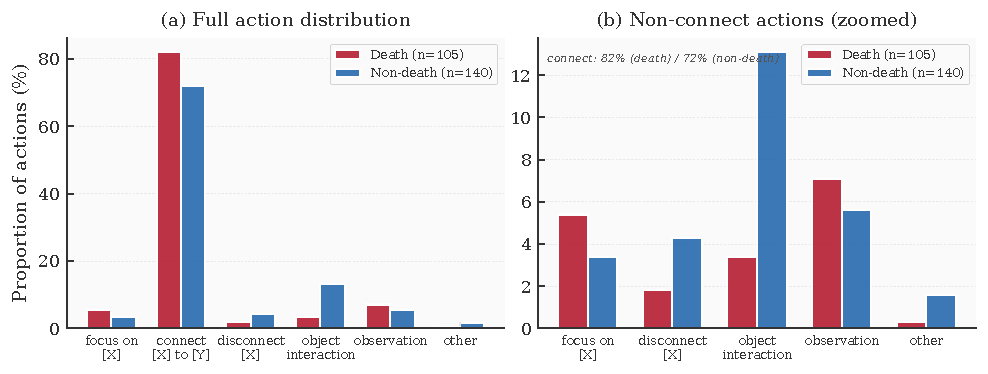
\includegraphics[width=\columnwidth]{figures/death_action_distribution.pdf}
\caption{Action distribution for the internal (LLM) strategy in death ($n{=}105$) vs.\ non-death ($n{=}140$) episodes. Left: full distribution (both dominated by \texttt{connect}). Right: non-\texttt{connect} actions zoomed. \texttt{focus on} is moderately more frequent in death episodes ($5.4\%$ vs.\ $3.4\%$), while non-death episodes show higher rates of observation and object interaction.}
\label{fig:death-action-dist}
\end{figure}

% Figure~\ref{fig:death-comparison} moved to main text (\S2)

\section{Grounding Ablation}
\label{app:grounding-ablation}

We test whether directly intervening on the dominant death action (\texttt{focus on}) eliminates death vulnerability on the 10 death-prone tasks (baseline 48.0\%, $n{=}200$).

\paragraph{Prompt warning.} Adding an explicit system prompt (``use \texttt{focus on} only for final answers'') reduces aggregate death rate to 37.0\% ($\Delta = -11$~pp). Both identification tasks exhibit ironic effects (\texttt{identify-life-stages-1}: 35\%$\to$50\%; \texttt{identify-life-stages-2}: 25\%$\to$70\%), where explicit mention of the dangerous action may have increased its salience.

\paragraph{Action-space filtering.} Blocking \texttt{focus on} during the exploration phase yields 379 blocks across 200 episodes with zero leaks and zero passthroughs (the agent never persisted in retrying blocked actions), reducing death rate to 29.0\% ($\Delta = -19$~pp). The zero-passthrough rate suggests \texttt{focus on} use is a shallow behavioral pattern rather than a deliberate strategy.

\paragraph{Per-task variation.} Under filtering, \texttt{identify-life-stages} and \texttt{inclined-plane} approach deterministic-level safety (${\sim}$15--20\% DR), while \texttt{chemistry-mix} and \texttt{find-animal} remain at 35--40\%. Residual deaths occur during the answer-submission window, where the filter is inactive and agents submit \texttt{focus on} to incorrect objects.

\paragraph{Post-ablation counterfactual decomposition.}
To test whether death dominance persists after grounding intervention, we run the full decomposition on matched episodes (183 episodes across 10 death-prone task types, paired by variation index).
Grounding reduces the internal death rate from 50.3\% to 35.0\% ($-15.3$\,pp), yet $\geq$93\% of disambiguating labels still arise from death asymmetry ($\Delta_\text{nd} \approx 0.09$, compared to $0.00$ at baseline).
Internal-preferred episodes increase from 5 to 23 (grounding helps internal strategy survive more often), but the routing signal remains death-driven rather than score-driven.
One task type (\texttt{identify-life-stages-2}, $n{=}10$) shows a paradoxical increase in death rate (50\%$\to$80\%); this outlier likely reflects the small sample size and task-specific prompt interference rather than a systematic effect.

\section{Ablation Studies}
\label{app:ablations}

\paragraph{Capacity scaling.} We scale the implicit router from Qwen3-0.6B to Qwen3-4B and evaluate at both step and episode level (Table~\ref{tab:capacity}).

\begin{table}[h]
\centering
\small
\begin{tabular}{@{}lcc@{}}
\toprule
Model & Step Bal.\ Acc.\ (\%) & Ep.\ Bal.\ Acc.\ (\%) \\
\midrule
Qwen3-0.6B & $56.4 \pm 3.5$ & $50.7 \pm 2.6$ \\
Qwen3-1.7B & $58.2 \pm 4.0$ & $43.1 \pm 1.0$ \\
Qwen3-4B & $59.2 \pm 3.5$ & $\mathbf{59.0 \pm 1.9}$ \\
\midrule
Always-det & 50.0 & 50.0 \\
\bottomrule
\end{tabular}
\caption{Capacity scaling: step-level and episode-level balanced accuracy (4 seeds, identical configuration across all scales). Step-level accuracy is flat ($56$--$59\%$, within seed variance). At episode level, only 4B breaks the random baseline ($59.0\%$, $p < 0.005$).}
\label{tab:capacity}
\end{table}

Step-level balanced accuracy is flat across scales ($56$--$59\%$, within seed variance); step-level discrimination is not capacity-sensitive. At episode level, only 4B breaks the random baseline ($59.0 \pm 1.9\%$, $p < 0.005$); 0.6B and 1.7B remain at or below chance. The 1.7B model's below-chance episode-level accuracy ($43.1\%$) may reflect overfitting to spurious step-level correlations that anti-correlate with episode outcomes; without per-class confusion matrices at this scale, this remains a hypothesis. The dominant explanation across scales is that death avoidance constitutes a task-type-level binary signal that a step-level router cannot exploit efficiently.

\paragraph{Generative router.} A generative routing model trained with explicit routing labels achieves balanced accuracy of 46.7\%, confirming that the routing bottleneck is signal-limited, not architecture-limited.

\paragraph{Leave-one-task-type-out routing.} Under leave-one-task-type-out evaluation, blind routing collapses to always-deterministic (balanced accuracy 50.0\%); a keyword-based variant achieves 62.9\% only through task-identity leakage, not genuine routing signal. A guided router evaluated under the same protocol confirms this: without task-type identifiers it achieves chance accuracy (50.0\%), and leaking task names raises this to 62.9\%, confirming that the only learnable routing feature is task-type identity.

\paragraph{Death-proximal labeling.} Training a router only on the $k$ steps preceding death events (rather than all steps) also collapses to majority-class prediction (step balanced accuracy 50.0\%, episode balanced accuracy 50.0\%, internal recall 0\%), confirming that the absence of step-level signal is not an artifact of label dilution across long episodes.

\paragraph{Reasoning depth.} An ablation comparing chain-of-thought reasoning against direct-answer generation on 6 task types ($n{=}120$ episodes per condition, 6 tasks $\times$ 20 episodes per task) found no significant difference (Mann--Whitney $p > 0.26$, $|d| \leq 0.31$) and near-identical death rates (41.8\% vs.\ 42.5\%); reasoning depth does not meaningfully alter internal-mode outcomes.

\section{Threshold Routing Analysis}
\label{sec:threshold-routing}

Given per-task death risk knowledge, we test whether a simple threshold routing strategy can outperform always-deterministic. For each threshold $t \in [0, 1]$, we route to internal if the per-task internal death rate $\leq t$, otherwise to deterministic, and sweep all thresholds to find the optimal.

\begin{table}[h]
\centering
\small
\resizebox{\columnwidth}{!}{%
\begin{tabular}{lccc}
\toprule
Strategy & Mean Score & Death Rate & $\Delta$ vs Det \\
\midrule
Always-det & $-9.47$ & $0.163$ & $0.00$ \\
Optimal threshold ($t{=}0$) & $-11.03$ & $0.155$ & $-1.56$ \\
Always-internal & $-39.07$ & $0.429$ & $-29.60$ \\
\bottomrule
\end{tabular}}
\caption{Death-risk threshold routing analysis on 245 episodes. The optimal threshold routes only \texttt{find-non-living-thing} (the sole zero-death task) to internal, with all other tasks routed to deterministic. Bootstrap 95\% CI for the difference: $[-8.87, +5.92]$.}
\label{tab:threshold-routing}
\end{table}

Even with perfect per-task death risk knowledge, threshold routing cannot outperform always-deterministic. The sole zero-death task achieves higher scores under deterministic (+28.5) than internal (+18.9), leaving no room for a beneficial mixed strategy.

\section{Practitioner Decision Framework}
\label{app:decision-framework}

Given a new interactive environment, the following three-stage procedure diagnoses whether learned routing adds value over a fixed deterministic strategy.

\paragraph{Stage 1: Pilot collection (${\sim}$50 episodes).}
Run pure-internal and pure-deterministic strategies on a representative sample (${\sim}$50 episode pairs). Compute the death-rate differential $\Delta\text{DR} = \text{DR}_{\text{int}} - \text{DR}_{\text{det}}$.

\paragraph{Stage 2: Death dominance check.}
If $\Delta\text{DR} > 15$~pp, death asymmetry is likely the dominant routing signal. Compute the death-label fraction $f_{\text{death}}$: the proportion of non-tie routing labels where exactly one strategy dies.

\paragraph{Stage 3: Decision.}
If $f_{\text{death}} > 75\%$, the routing signal is death-dominated; a fixed deterministic strategy will match or exceed any learned router. If $f_{\text{death}} < 50\%$, diverse routing signals may justify a learned router. Between 50\%--75\%, collect additional episodes to reduce estimation noise before committing to router development.

\paragraph{Retrospective validation.}
All four experimental conditions in this paper are correctly classified:

\begin{table}[h]
\centering
\small
\begin{tabular}{@{}lrrll@{}}
\toprule
Condition & $\Delta$DR & $f_{\text{death}}$ & Prediction & Actual \\
\midrule
Qwen-7B & +26.5 & 78.9\% & det-fixed & det wins \\
Llama-8B & +30.0 & $>$75\% & det-fixed & det wins \\
Qwen-72B & +27.8 & $>$75\% & det-fixed & det wins \\
MATH & +0.5 & 0\% & router viable & no signal \\
\bottomrule
\end{tabular}
\caption{Retrospective validation of the decision framework. All four conditions are correctly classified (4/4).}
\label{tab:decision-framework}
\end{table}

The framework also predicts the inverted-U relationship between capability and death risk: below ${\sim}$0.5B parameters, agents rarely reach dangerous states (13.3\% death rate in a 15-episode pilot), so $\Delta\text{DR}$ is low and the framework would not recommend fixed-deterministic. Above ${\sim}$7B, agents are capable enough to enter catastrophic states but not capable enough to avoid them, producing high $\Delta\text{DR}$.

\paragraph{Threshold calibration.} The thresholds above (15~pp, 75\%, 50\%) are illustrative, derived from ScienceWorld's specific reward structure (binary death penalty $P{=}100$, sparse terminal rewards). Environments with graded penalties, dense rewards, or qualitatively different failure modes may require different thresholds. Practitioners should calibrate these boundaries for their specific environment.

\section{Extended Validation of Excluded Tasks}
\label{app:extended-validation}

To verify that task exclusion does not bias toward death-prone tasks, we collect $n{=}20$ episodes for five representative excluded tasks spanning all exclusion categories (Table~\ref{tab:extended-val}).

\begin{table}[h]
\centering
\small
\resizebox{\columnwidth}{!}{%
\begin{tabular}{lcrrrrc}
\toprule
Task & Category & $n$ & Int DR & Det DR & $\Delta$DR & D/I/N \\
\midrule
boil & dev-set & 20 & 55\% & 25\% & +30\,pp & 6/0/14 \\
melt & dev-set & 20 & 45\% & 20\% & +25\,pp & 7/2/11 \\
find-living-thing & taxonomic & 20 & 55\% & 15\% & +40\,pp & 10/0/10 \\
use-thermometer & agent-floor & 20 & 50\% & 20\% & +30\,pp & 7/1/12 \\
power-component & agent-floor & 20 & 50\% & 15\% & +35\,pp & 7/0/13 \\
\midrule
\textit{Mean (5 tasks)} & & 100 & 51.0\% & 19.0\% & +32.0\,pp & 37/3/60 \\
\bottomrule
\end{tabular}}
\caption{Extended validation ($n{=}20$) of representative excluded task types. All five tasks confirm death asymmetry; mean $\Delta$DR $= +32.0$\,pp is consistent with the $n{=}5$ prescreening estimate for these same tasks (Table~\ref{tab:excluded-death}).}
\label{tab:extended-val}
\end{table}

Notably, the excluded-task aggregate DAF (0.991) exceeds the included-task DAF (0.904; Table~\ref{tab:per-task}), indicating that excluded tasks are \emph{more} death-dominated than included tasks, the opposite of a cherry-picking bias.

\section{Agent Prompt Templates}
\label{app:prompt-templates}

Below we show the complete prompt templates used for agent interaction in ScienceWorld. Both the internal (ReAct) and deterministic strategies share the same system prompt but differ in the user message template.

\paragraph{System prompt (shared).} Used for all ScienceWorld agent interactions across both computation modes.

\begin{tcblisting}{listing only, colback=gray!5!white, colframe=gray!75!black,
  listing options={basicstyle=\small\ttfamily,breaklines=true,columns=fullflexible},
  left=2mm, right=2mm, top=1mm, bottom=1mm}
You are an agent interacting with a ScienceWorld text
environment. Your goal is to complete the given task by
choosing actions from the available action list.

Use the following format for each step:
Thought: <your reasoning about what to do next>
Action: <exact action string from the valid actions list>

Rules:
- You MUST choose an action from the valid actions list.
  Do not invent actions.
- Think step by step about what physical/scientific
  process is needed.
- Pay attention to the current observation for clues
  about object states.
\end{tcblisting}

\paragraph{Internal (ReAct) user template.} At each step, the agent receives the current observation, valid action list, and recent action history, and must select a single action.

\begin{tcblisting}{listing only, colback=gray!5!white, colframe=gray!75!black,
  listing options={basicstyle=\small\ttfamily,breaklines=true,columns=fullflexible},
  left=2mm, right=2mm, top=1mm, bottom=1mm}
Current observation:
{observation}

Valid actions:
{valid_actions_str}

Previous actions taken: {history_str}

Choose your next action.
\end{tcblisting}

\paragraph{Deterministic candidate generation template.} For the deterministic strategy, the agent generates ranked candidate actions instead of selecting one; these candidates are then evaluated via simulator forking (\S\ref{sec:method}).

\begin{tcblisting}{listing only, colback=gray!5!white, colframe=gray!75!black,
  listing options={basicstyle=\small\ttfamily,breaklines=true,columns=fullflexible},
  left=2mm, right=2mm, top=1mm, bottom=1mm}
Current observation:
{observation}

Valid actions:
{valid_actions_str}

Previous actions taken: {history_str}

Generate the top 3 most promising actions from the valid
actions list, ranked by how likely they are to make
progress on the task. Output exactly 3 actions, one per
line, in this format:
1. <action>
2. <action>
3. <action>
\end{tcblisting}

\paragraph{Reflexion self-reflection prompt.} After a failed episode, the Reflexion agent (\S\ref{sec:agent-improvement}) generates a reflection that is injected into subsequent trial attempts as additional system context.

\begin{tcblisting}{listing only, colback=gray!5!white, colframe=gray!75!black,
  listing options={basicstyle=\small\ttfamily,breaklines=true,columns=fullflexible},
  left=2mm, right=2mm, top=1mm, bottom=1mm}
You just completed an episode in a ScienceWorld text
environment but failed.

Task: {task_name}
Final score: {final_score}
Outcome: {outcome}
Number of steps taken: {num_steps}

Here is a summary of your actions:
{action_summary}

Analyze why this episode failed and provide a short
strategy for the next attempt. Focus on:
1. What went wrong (wrong sequence, missed key step,
   dangerous action)?
2. What should be done differently next time?

Keep your reflection under 200 words.
\end{tcblisting}

\paragraph{Grounding warning (ablation).} The prompt warning condition in the grounding ablation (Appendix~\ref{app:grounding-ablation}) appends the following to the shared system prompt:

\begin{tcblisting}{listing only, colback=gray!5!white, colframe=gray!75!black,
  listing options={basicstyle=\small\ttfamily,breaklines=true,columns=fullflexible},
  left=2mm, right=2mm, top=1mm, bottom=1mm}
CRITICAL SAFETY RULE: The 'focus on [object]' action is
ONLY for submitting your final answer. Do NOT use
'focus on' to examine, inspect, or interact with objects
during exploration. Using 'focus on' on the wrong object
will cause irreversible failure. Use 'look at',
'examine', or 'pick up' instead for exploration.
\end{tcblisting}

\noindent The key difference between the two computation modes is the user message: the internal strategy asks the LLM to \emph{select} one action (ReAct), while the deterministic strategy asks it to \emph{rank} candidates for simulator evaluation. Both use identical system prompts and identical observation formatting.

\section{Non-Death Episode Case Study}
\label{app:non-death-case-study}

We illustrate the framework's ability to decompose non-death routing signal using \texttt{find-non-living-thing}, the only task type with zero deaths and 100\% non-death labels (\S\ref{sec:death-decomp}). Using Gemma-2-9B-it counterfactual episodes ($N{=}20$), 12 episodes show routing preference (9 deterministic-preferred, 3 internal-preferred), confirming the framework detects bidirectional signal independent of death asymmetry.

\paragraph{Deterministic-preferred: knowledge retrieval advantage.}
In Episode~3 (det: 67, int: 0), the internal strategy issues nonsensical \texttt{connect} actions for 18 consecutive steps (e.g., ``connect air to outside,'' ``connect axe to door to foundry'') without ever identifying a target object; the deterministic strategy correctly focuses on ``orange'' (+58) and opens the kitchen door (+9). In Episode~17 (det: 58, int: 50), both strategies find a valid non-living thing, but the deterministic strategy selects a higher-scoring object (orange, 58\,pts) versus the internal strategy's choice (fountain, 50\,pts), illustrating that object selection quality creates routing signal even when both strategies succeed.

\paragraph{Internal-preferred: semantic reasoning advantage.}
In Episode~12 (int: 67, det: 58), the task specifies ``move it to the red box in the living room.'' The deterministic strategy focuses on the red box itself, the destination container, not a separate non-living thing, scoring 58\,pts. The internal strategy correctly distinguishes target from container, choosing ``orange'' (67\,pts). This semantic error demonstrates that deterministic pattern-matching can miss task-structure subtleties that internal reasoning captures.

These cases confirm two properties: (1)~the framework captures non-death routing signal when it exists, and (2)~signal flows in both directions: neither strategy uniformly dominates in death-free tasks.

\paragraph{Systematic analysis of non-death labels.}
All 20 non-death non-tie labels in the primary Qwen2.5-7B analysis originate from \texttt{find-non-living-thing}, the sole death-free task type. In every other task type, non-tie episodes involve at least one strategy dying. We classify the 20 episodes into three error categories:

\begin{table}[h]
\centering
\small
\begin{tabular}{@{}lrrr@{}}
\toprule
Error category & Det-pref & Int-pref & Total \\
\midrule
Hallucination-induced & 8 & 2 & 10 \\
Object selection quality & 6 & 1 & 7 \\
Action selection error & 2 & 1 & 3 \\
\bottomrule
\end{tabular}
\caption{Non-death non-tie episode classification. Hallucination-induced: agent's state model is incorrect (e.g., believing \texttt{eat} completes the task). Object selection quality: both strategies succeed but choose different-value objects. Action selection: correct state model but suboptimal action sequences.}
\label{tab:non-death-taxonomy}
\end{table}

\noindent Hallucination-induced errors dominate (50\%), driven by a recurring ``eat before focus'' pattern: the internal strategy consumes the target object (destroying it) before attempting the scoring action (\texttt{focus on}), indicating an incorrect state model that equates eating with task completion (11 of 20 episodes). Object selection quality accounts for 35\%: typically the deterministic strategy selecting ``orange'' (58\,pts) while the internal strategy settles for lower-value objects (``fountain'' or ``picture,'' 50\,pts). The error categories are bidirectional: 2 of 10 hallucination episodes and 1 of 3 action selection episodes are internal-preferred, confirming the framework detects failures in both strategies. Score gaps reflect category severity: hallucination errors produce large gaps ($17$--$67$\,pts, one strategy scores zero) while object selection differences produce small gaps ($8$--$9$\,pts, both strategies functional).

\section{Use of AI Assistance}
We used Claude for coding, code drafting, debugging, and language polishing.

\end{document}
